% Sección del informe: experimentos (entregables 2, 3, 4, 5 y 6).
% Uso en el main.tex de NeurIPS:  % Sección del informe: experimentos (entregables 2, 3, 4, 5 y 6).
% Uso en el main.tex de NeurIPS:  % Sección del informe: experimentos (entregables 2, 3, 4, 5 y 6).
% Uso en el main.tex de NeurIPS:  % Sección del informe: experimentos (entregables 2, 3, 4, 5 y 6).
% Uso en el main.tex de NeurIPS:  \input{experimentos}   (requiere \usepackage{booktabs} y \usepackage{graphicx})
% Fuente de los números: output-train/ (versión de knee-train del 27 oct 2026, GPU T4, 15 épocas, 49 min en total).

\section{Experimentos}
\label{sec:experimentos}

\paragraph{Protocolo.}
Del total de estudios sin etiqueta experta se tomó un subconjunto estratificado de 600: se incluyen primero los positivos débiles de los hallazgos raros.
De ellos, 540 se usan para entrenar y 60 forman un \emph{holdout}; la partición se hace por reporte, para que dos estudios con el mismo texto no queden en lados distintos.
El holdout tiene solo etiquetas débiles y se usa para elegir la época y los umbrales.
Los 58 estudios gold se excluyen del entrenamiento y solo se usan para la evaluación final.
Cada estudio se representa con una serie por plano (sagital, coronal y axial), 16 cortes de $224\times224$ y ventanas 2.5D de tres cortes vecinos.
En entrenamiento se muestrean 8 ventanas por plano; en evaluación se usan todas.
Los aumentos son rotación $\pm10^\circ$, escala $\pm10\%$ y gamma, sin espejado horizontal (medial y lateral son parte del diagnóstico).
La optimización usa AdamW (tasa $10^{-4}$ en el \emph{backbone} y $10^{-3}$ en la cabeza, \emph{weight decay} $10^{-2}$), calentamiento del $5\%$, decaimiento coseno, recorte de gradiente en $1$ y precisión mixta.
Se entrena 15 épocas con lotes de 8 (4 para ResNet-50) y se conserva la época con mejor AUC macro en el holdout.
Los 7 experimentos tardaron 49 min en una GPU T4.
Los intervalos de confianza (IC 95\%) se obtienen con 1000 remuestreos \emph{bootstrap} de los 58 estudios gold; para las diferencias se usa un bootstrap pareado contra la referencia \texttt{B\_resnet18}.

\begin{table}[t]
  \caption{Resultados en los 58 estudios gold. $\Delta$: diferencia de AUC macro contra la referencia B, con IC 95\% pareado.
    F1 macro con el umbral elegido en el holdout. Época: la de mejor AUC en holdout (de 0 a 14).}
  \label{tab:experimentos}
  \centering
  \small
  \setlength{\tabcolsep}{4pt}
  \begin{tabular}{@{}llccccccc@{}}
    \toprule
    & Variación & AUC gold & IC 95\% & $\Delta$ vs B & IC 95\% $\Delta$ & F1 & Época & Min \\
    \midrule
    A & CNN desde cero         & .589 & [.525, .647] & $-.140$ & [$-.198$, $-.078$] & .447 &  4 &  5.8 \\
    B & ResNet-18 ImageNet (ref.) & .729 & [.673, .782] & ---  & ---                  & .554 & 10 &  5.1 \\
    C & pérdida focal          & .740 & [.686, .789] & $+.011$ & [$-.017$, $+.040$] & .550 &  7 &  5.1 \\
    D & solo etiquetas seguras & .707 & [.648, .761] & $-.022$ & [$-.064$, $+.020$] & .530 & 13 &  5.1 \\
    E & solo plano sagital     & .734 & [.681, .784] & $+.005$ & [$-.046$, $+.052$] & .527 & 14 &  1.9 \\
    F & sin \texttt{pos\_weight} & .737 & [.684, .787] & $+.008$ & [$-.023$, $+.040$] & .553 & 13 &  5.1 \\
    G & ResNet-50 ImageNet     & .741 & [.690, .793] & $+.012$ & [$-.021$, $+.048$] & .551 & 10 & 13.4 \\
    \bottomrule
  \end{tabular}
\end{table}

\paragraph{CNN desde cero frente a transfer learning (entregable 2).}
Ambas arquitecturas comparten la cabeza (proyección, codificación de plano y posición, dos bloques de autoatención y 12 consultas de atención, una por hallazgo, con 12 sigmoides independientes) y solo cambian el extractor de rasgos.
La CNN desde cero (A, 3.1 M parámetros, 5 bloques estilo VGG~\cite{simonyan2015vgg}) obtiene un AUC de $0.589$.
ResNet-18 preentrenada en ImageNet~\cite{he2016resnet} (B, 13.2 M parámetros) llega a $0.729$.
La diferencia, $-0.140$ [$-0.198$, $-0.078$], es la única de la Tabla~\ref{tab:experimentos} cuyo intervalo excluye el cero.
La Figura~\ref{fig:experimentos} muestra por qué: la CNN desde cero alcanza su mejor holdout en la época 4 y luego se estanca alrededor de $0.58$, aunque su pérdida de entrenamiento sigue bajando lentamente.
Con 540 estudios y etiquetas ruidosas no aprende rasgos que generalicen.
Los modelos preentrenados mejoran hasta las épocas 7--10 y luego se estabilizan, lo que indica que 15 épocas fueron suficientes.

\begin{figure}[t]
  \centering
  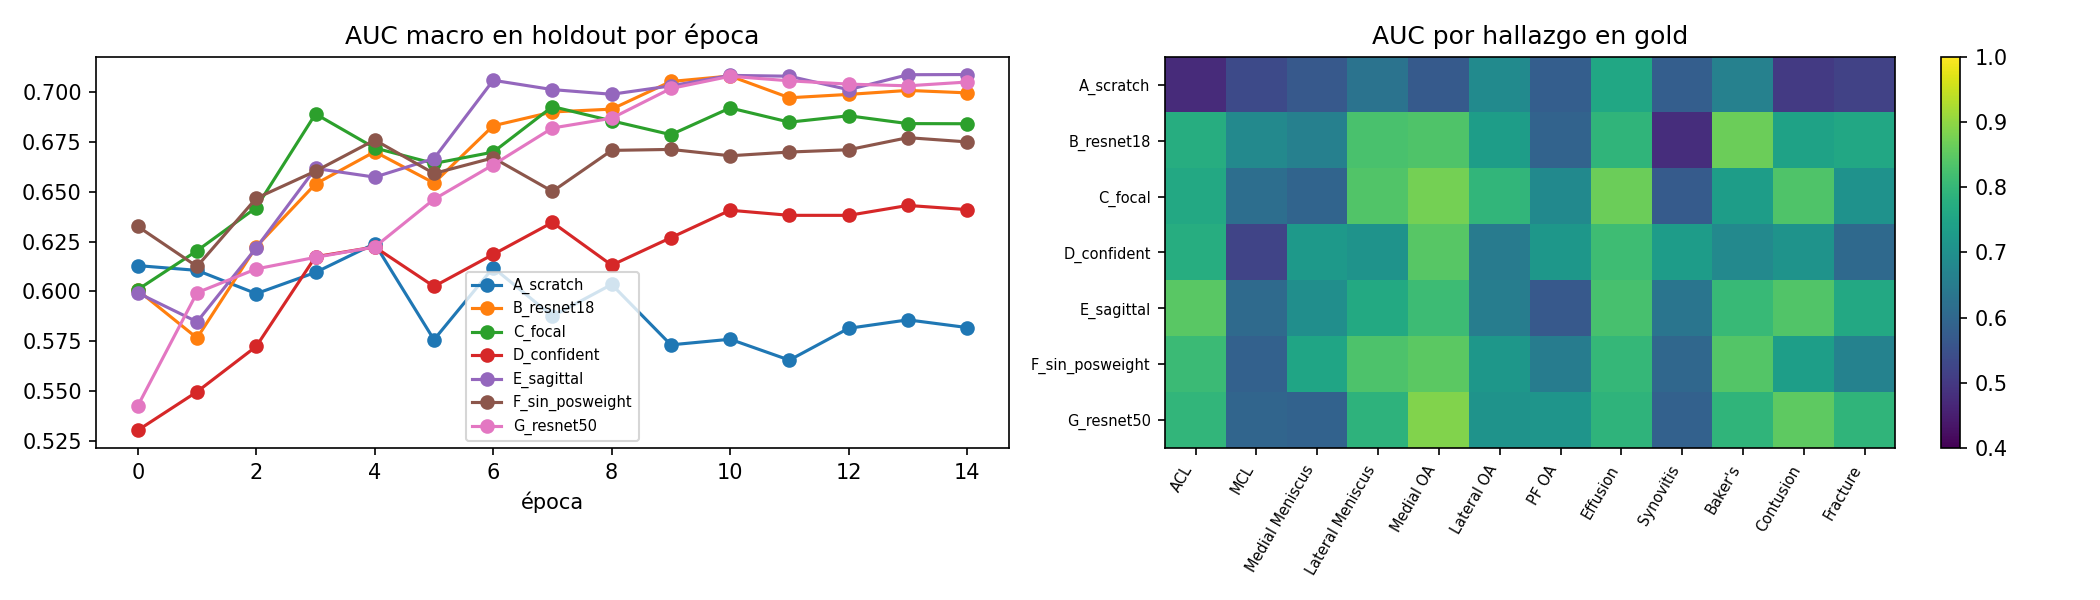
\includegraphics[width=\linewidth]{figs/experimentos.png}
  \caption{Izquierda: AUC macro en el holdout por época. Derecha: AUC por hallazgo en los gold para cada experimento.}
  \label{fig:experimentos}
\end{figure}

\paragraph{Ablaciones (entregable 4).}
Ninguna de las cinco variaciones sobre B produce una diferencia significativa: todos los intervalos de $\Delta$ incluyen el cero.
Con 58 estudios gold, diferencias de AUC menores a $\sim0.04$ no se pueden distinguir del azar, así que las conclusiones siguientes son tendencias.
\begin{itemize}
  \item \textbf{Pérdida} (C, focal~\cite{lin2017focal}, $\gamma=2$): $+0.011$. Es el mejor modelo en derrame ($0.865$) y contusión ($0.835$).
  \item \textbf{Manejo de etiquetas ruidosas} (D): descartar el silencio y las dudas (peso $0$) en lugar de ponderarlos ($0.3$ y $0.5$) baja el AUC macro ($-0.022$), pero cambia mucho según el hallazgo. En sinovitis, D llega a $0.732$ frente a $0.479$ de B. El extractor menciona la sinovitis en solo el $36\%$ de los reportes y el experto la marca en el $47\%$ de los gold, de modo que tratar el silencio como negativo le enseña a B que la sinovitis casi nunca está presente. El mismo efecto, menor, aparece en artrosis patelofemoral ($0.717$ frente a $0.592$) y menisco medial ($0.721$ frente a $0.662$). En cambio, D empeora en MCL, quiste de Baker y fractura, donde descartar el silencio deja muy pocos ejemplos.
  \item \textbf{Plano} (E, solo sagital): rinde igual que los tres planos ($+0.005$) en el $37\%$ del tiempo. El resultado es coherente con la práctica clínica: el ligamento cruzado anterior se evalúa en el plano sagital y E es el mejor modelo en ACL ($0.847$), mientras que pierde en artrosis patelofemoral ($0.568$) y lateral ($0.654$), que se ven mejor en los planos axial y coronal.
  \item \textbf{Profundidad del backbone} (G, ResNet-50): $+0.012$ a 2.6 veces el costo. Es el mejor AUC macro ($0.741$), pero la mejora no es significativa.
\end{itemize}

\begin{table}[t]
  \caption{AUC por hallazgo en los gold. Última columna: el extractor de texto (v4, Sección~\ref{sec:extractor}), que generó las etiquetas de entrenamiento.
    $n^{+}$: positivos según el experto.}
  \label{tab:auc-hallazgo}
  \centering
  \small
  \setlength{\tabcolsep}{4pt}
  \begin{tabular}{@{}lrccccccc|c@{}}
    \toprule
    Hallazgo & $n^{+}$ & A & B & C & D & E & F & G & Texto \\
    \midrule
    ACL              & 24 & .474 & .775 & .761 & .775 & .847 & .809 & .795 & .885 \\
    MCL              &  9 & .535 & .683 & .617 & .524 & .608 & .587 & .596 & .754 \\
    Medial Meniscus  & 26 & .569 & .662 & .594 & .721 & .696 & .754 & .588 & .752 \\
    Lateral Meniscus & 23 & .629 & .827 & .837 & .709 & .764 & .832 & .788 & .806 \\
    Medial OA        & 15 & .571 & .836 & .874 & .843 & .811 & .850 & .885 & .760 \\
    Lateral OA       & 11 & .687 & .733 & .795 & .650 & .654 & .718 & .708 & .733 \\
    PF OA            & 21 & .579 & .592 & .685 & .717 & .568 & .651 & .713 & .690 \\
    Effusion         & 35 & .758 & .793 & .865 & .814 & .825 & .799 & .790 & .666 \\
    Synovitis        & 27 & .579 & .479 & .572 & .732 & .633 & .600 & .587 & .658 \\
    Baker's          & 12 & .663 & .864 & .734 & .683 & .804 & .841 & .792 & .821 \\
    Contusion        & 19 & .502 & .745 & .835 & .707 & .837 & .735 & .852 & .760 \\
    Fracture         & 18 & .519 & .760 & .707 & .606 & .761 & .665 & .793 & .758 \\
    \midrule
    Macro            &    & .589 & .729 & .740 & .707 & .734 & .737 & .741 & .753 \\
    \bottomrule
  \end{tabular}
\end{table}

\paragraph{Resultados por hallazgo (entregable 3).}
La Tabla~\ref{tab:auc-hallazgo} compara cada modelo con el extractor de texto que generó sus etiquetas.
En promedio, el mejor modelo de imagen ($0.741$) queda cerca de su ``maestro'' ($0.753$).
En varios hallazgos lo supera: derrame ($0.865$ en C frente a $0.666$), artrosis medial ($0.885$ en G frente a $0.760$), contusión ($0.852$ en G frente a $0.760$) y menisco lateral ($0.837$ en C frente a $0.806$).
Un modelo entrenado con etiquetas ruidosas puede superar a la fuente de esas etiquetas cuando el ruido no es sistemático, porque la red promedia los errores individuales~\cite{ratner2017snorkel}.
Para ACL, MCL y sinovitis ocurre lo contrario: el reporte describe el hallazgo de forma más directa de lo que la imagen permite aprender con 540 estudios.
El AUC por hallazgo se apoya en 9 a 35 positivos, por lo que sus intervalos son amplios (no mostrados).

\paragraph{Umbral y métricas de decisión.}
El modelo final se elige sin mirar los gold: es el de mejor AUC en el holdout, \texttt{E\_sagittal} ($0.7087$, empatado en la práctica con B y G).
Para cada hallazgo, el umbral es el que maximiza F1 en el holdout.
Elegirlo en los gold daría métricas optimistas, porque se estaría ajustando sobre el mismo conjunto en que se evalúa.
La Tabla~\ref{tab:prf} muestra el resultado.
El recall medio ($0.73$) es mayor que la precisión ($0.47$) porque la prevalencia de los gold difiere de la del entrenamiento (Tabla~\ref{tab:prevalencia}).
Un umbral elegido con la prevalencia débil no se traslada bien a los gold: en sinovitis y fractura, que son mucho más frecuentes en los gold, el recall cae a $0.22$ y $0.33$.

\begin{table}[t]
  \caption{Modelo final (\texttt{E\_sagittal}, elegido por holdout) en los gold, con umbrales que maximizan F1 en el holdout.}
  \label{tab:prf}
  \centering
  \small
  \begin{tabular}{@{}lcccccc@{}}
    \toprule
    Hallazgo & Prevalencia gold & AUC & Umbral & Precisión & Recall & F1 \\
    \midrule
    ACL              & .414 & .847 & .64 & .750 & .750 & .750 \\
    MCL              & .155 & .608 & .53 & .167 & .444 & .242 \\
    Medial Meniscus  & .448 & .696 & .20 & .491 & 1.00 & .658 \\
    Lateral Meniscus & .397 & .764 & .08 & .543 & .826 & .655 \\
    Medial OA        & .259 & .811 & .26 & .361 & .867 & .510 \\
    Lateral OA       & .190 & .654 & .11 & .211 & .727 & .327 \\
    PF OA            & .362 & .568 & .20 & .358 & .905 & .514 \\
    Effusion         & .603 & .825 & .43 & .660 & .943 & .776 \\
    Synovitis        & .466 & .633 & .61 & .667 & .222 & .333 \\
    Baker's          & .207 & .804 & .27 & .300 & 1.00 & .462 \\
    Contusion        & .328 & .837 & .78 & .600 & .789 & .682 \\
    Fracture         & .310 & .761 & .84 & .545 & .333 & .414 \\
    \midrule
    Media            &      & .734 &     & .471 & .734 & .527 \\
    \bottomrule
  \end{tabular}
\end{table}

\begin{table}[t]
  \caption{Prevalencia por hallazgo: etiquetas débiles (train y holdout, puntaje $\geq 0.5$) frente a los gold.}
  \label{tab:prevalencia}
  \centering
  \small
  \begin{tabular}{@{}lcccr@{}}
    \toprule
    Hallazgo & Train (débil) & Holdout (débil) & Gold & $n^{+}$ gold \\
    \midrule
    Fracture         & .128 & .083 & .310 & 18 \\
    Contusion        & .167 & .183 & .328 & 19 \\
    MCL              & .193 & .183 & .155 &  9 \\
    Lateral Meniscus & .202 & .283 & .397 & 23 \\
    Synovitis        & .226 & .217 & .466 & 27 \\
    ACL              & .231 & .317 & .414 & 24 \\
    Baker's          & .283 & .350 & .207 & 12 \\
    Lateral OA       & .359 & .500 & .190 & 11 \\
    Medial Meniscus  & .415 & .500 & .448 & 26 \\
    Medial OA        & .431 & .450 & .259 & 15 \\
    PF OA            & .481 & .650 & .362 & 21 \\
    Effusion         & .613 & .617 & .603 & 35 \\
    \bottomrule
  \end{tabular}
\end{table}

\paragraph{Desbalance de clases (entregable 6).}
En las etiquetas débiles de entrenamiento, la prevalencia va del $13\%$ (fractura) al $61\%$ (derrame) (Tabla~\ref{tab:prevalencia}).
Como mitigación principal, la BCE usa \texttt{pos\_weight} $=(1-p)/p$ por hallazgo, acotado a $[1, 10]$; como alternativa se evaluó la pérdida focal.
Quitar \texttt{pos\_weight} (F) no empeora el AUC ($+0.008$).
Esto es esperable: el AUC solo mide el orden de los casos, y \texttt{pos\_weight} sobre todo desplaza la calibración, lo que aquí se compensa al elegir el umbral en el holdout.
F tiene más recall y menos precisión que B.
La focal (C) da una mejora pequeña y no significativa.
El desbalance que más afecta al resultado no es el interno, sino el desplazamiento entre las etiquetas débiles y los gold.
Fractura, contusión y sinovitis tienen en los gold el doble de prevalencia que en el entrenamiento, y las artrosis lateral y medial casi la mitad.
Los gold parecen haber sido elegidos con más patología, y además el extractor sub-registra los hallazgos que el reporte omite.

\begin{figure}[t]
  \centering
  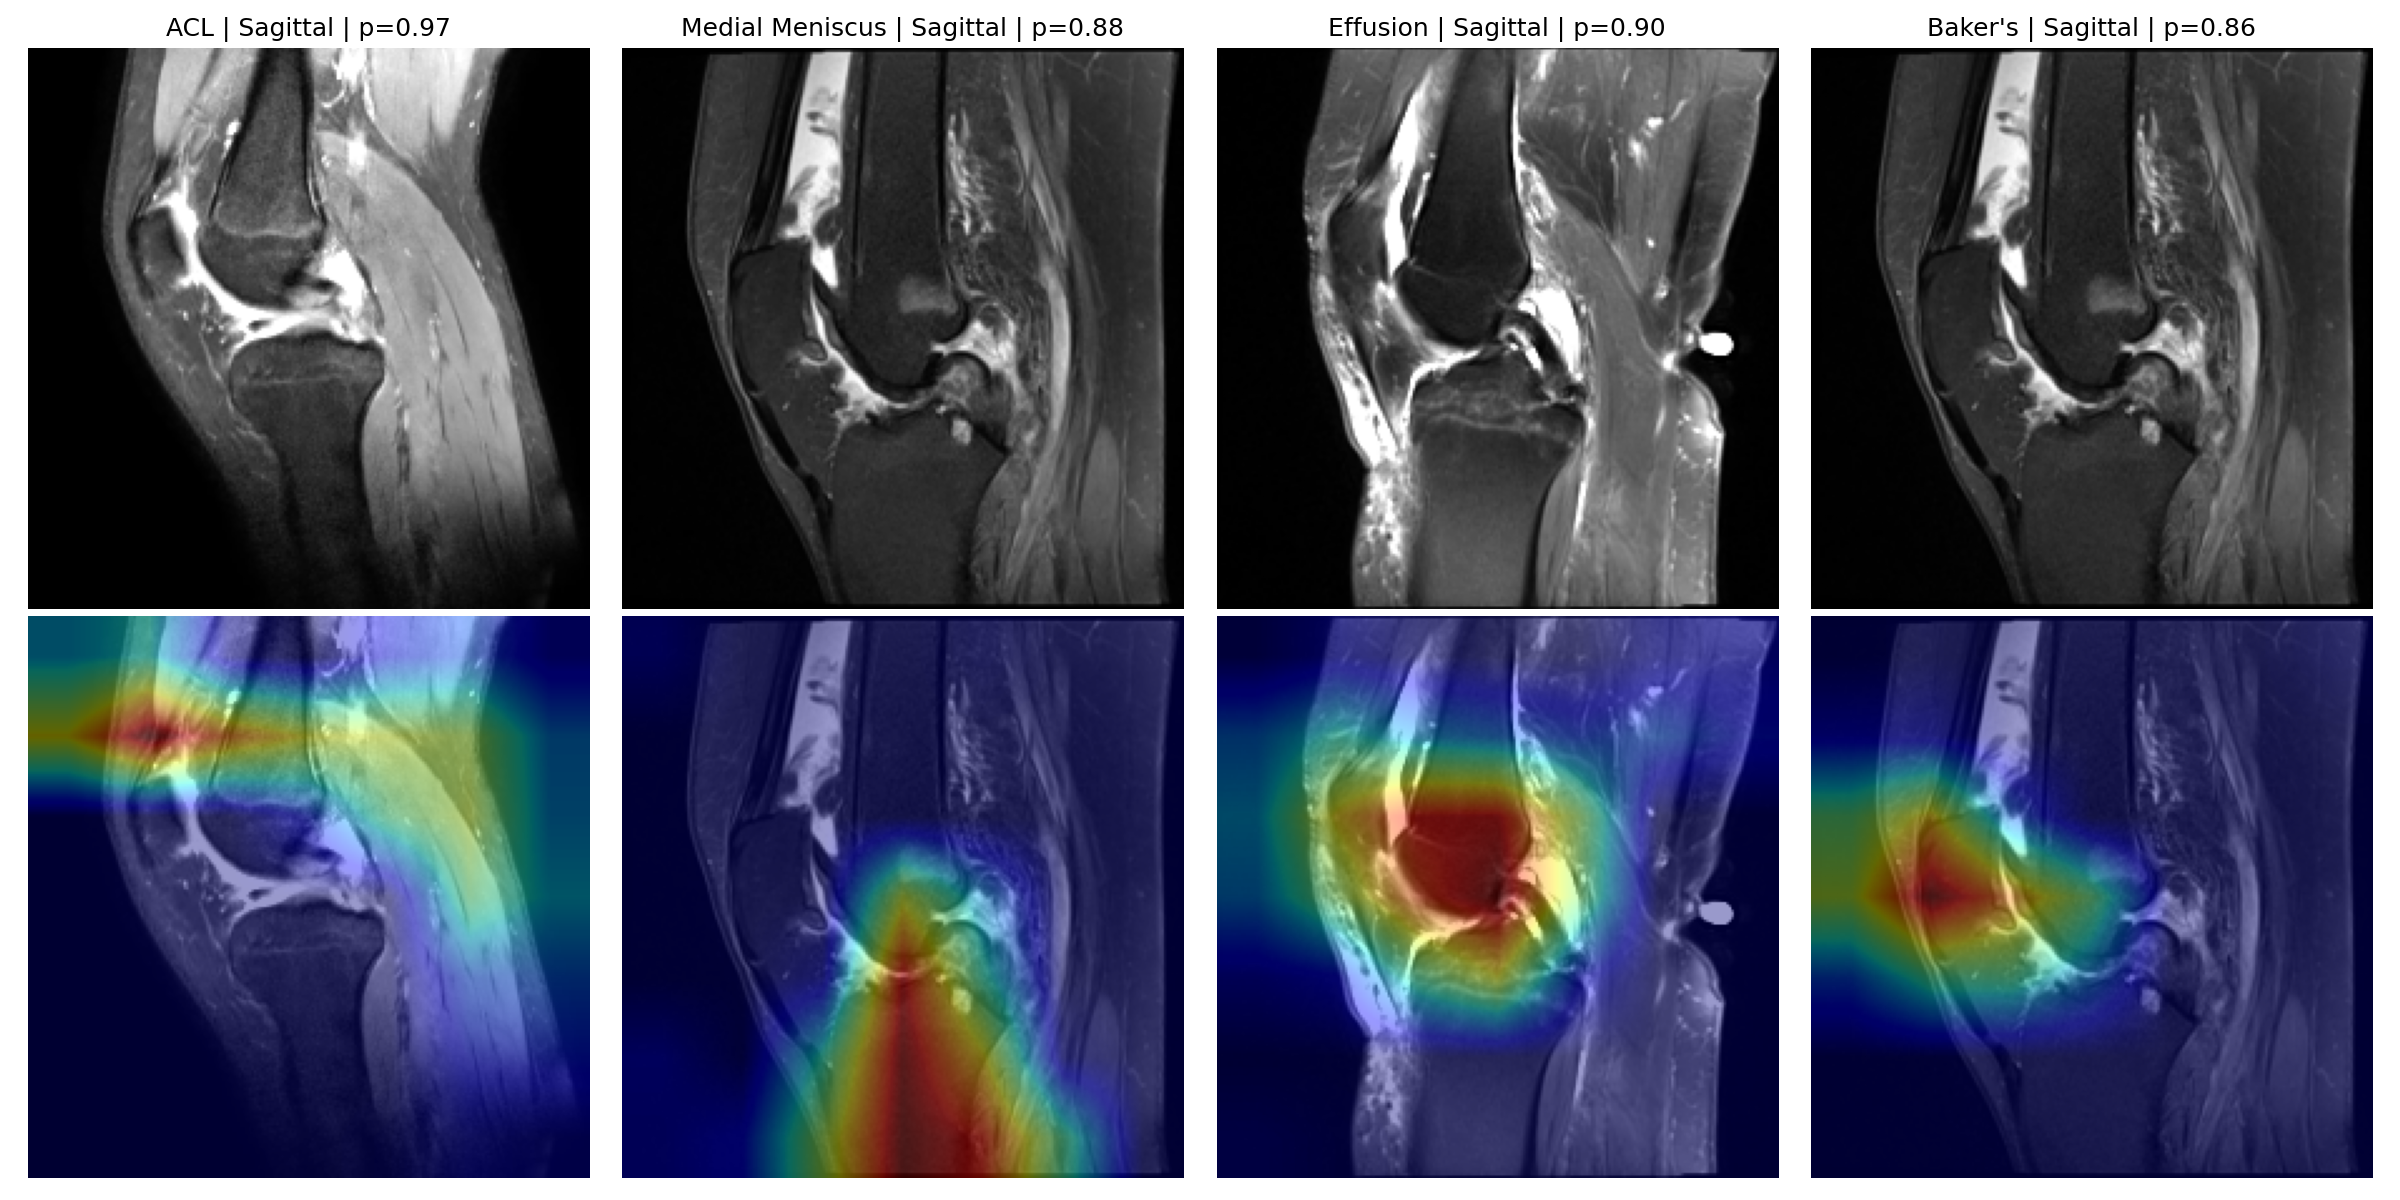
\includegraphics[width=\linewidth]{figs/gradcam.png}
  \caption{Grad-CAM del modelo final (\texttt{E\_sagittal}) sobre la última capa convolucional, en la ventana con mayor atención para cada hallazgo y un estudio gold positivo.
    En las imágenes, anterior está a la izquierda.}
  \label{fig:gradcam}
\end{figure}

\paragraph{Interpretabilidad (entregable 5).}
La Figura~\ref{fig:gradcam} aplica Grad-CAM~\cite{selvaraju2017gradcam} a cuatro hallazgos.
Solo el mapa del derrame es anatómicamente plausible: cubre la cavidad articular y el receso anterior al fémur.
El del menisco medial parte de la línea articular, donde está el menisco, pero se extiende hacia la diáfisis tibial.
Los de ACL y quiste de Baker no señalan la estructura correcta.
El de ACL se concentra en la región suprarrotuliana anterior y no en la escotadura intercondílea.
El de Baker se concentra en la grasa de Hoffa, en la cara anterior, mientras que el quiste poplíteo es posterior.
En la corrida de prueba de una época, el mapa de Baker también apuntaba a la región anterior.
Una explicación plausible es un atajo por co-ocurrencia.
La rotura aguda de ACL suele acompañarse de derrame (hemartrosis), y el quiste de Baker comunica con el líquido articular.
Como las etiquetas débiles salen del mismo reporte, el modelo puede aprender a predecir esos hallazgos a partir del líquido articular, que es más fácil de ver.
El AUC de ACL ($0.847$) sería entonces en parte un efecto de correlación y no de reconocer el ligamento.
Además, la resolución de Grad-CAM en la última capa de ResNet es de $7\times7$, por lo que la localización es gruesa.
   (requiere \usepackage{booktabs} y \usepackage{graphicx})
% Fuente de los números: output-train/ (versión de knee-train del 27 oct 2026, GPU T4, 15 épocas, 49 min en total).

\section{Experimentos}
\label{sec:experimentos}

\paragraph{Protocolo.}
Del total de estudios sin etiqueta experta se tomó un subconjunto estratificado de 600: se incluyen primero los positivos débiles de los hallazgos raros.
De ellos, 540 se usan para entrenar y 60 forman un \emph{holdout}; la partición se hace por reporte, para que dos estudios con el mismo texto no queden en lados distintos.
El holdout tiene solo etiquetas débiles y se usa para elegir la época y los umbrales.
Los 58 estudios gold se excluyen del entrenamiento y solo se usan para la evaluación final.
Cada estudio se representa con una serie por plano (sagital, coronal y axial), 16 cortes de $224\times224$ y ventanas 2.5D de tres cortes vecinos.
En entrenamiento se muestrean 8 ventanas por plano; en evaluación se usan todas.
Los aumentos son rotación $\pm10^\circ$, escala $\pm10\%$ y gamma, sin espejado horizontal (medial y lateral son parte del diagnóstico).
La optimización usa AdamW (tasa $10^{-4}$ en el \emph{backbone} y $10^{-3}$ en la cabeza, \emph{weight decay} $10^{-2}$), calentamiento del $5\%$, decaimiento coseno, recorte de gradiente en $1$ y precisión mixta.
Se entrena 15 épocas con lotes de 8 (4 para ResNet-50) y se conserva la época con mejor AUC macro en el holdout.
Los 7 experimentos tardaron 49 min en una GPU T4.
Los intervalos de confianza (IC 95\%) se obtienen con 1000 remuestreos \emph{bootstrap} de los 58 estudios gold; para las diferencias se usa un bootstrap pareado contra la referencia \texttt{B\_resnet18}.

\begin{table}[t]
  \caption{Resultados en los 58 estudios gold. $\Delta$: diferencia de AUC macro contra la referencia B, con IC 95\% pareado.
    F1 macro con el umbral elegido en el holdout. Época: la de mejor AUC en holdout (de 0 a 14).}
  \label{tab:experimentos}
  \centering
  \small
  \setlength{\tabcolsep}{4pt}
  \begin{tabular}{@{}llccccccc@{}}
    \toprule
    & Variación & AUC gold & IC 95\% & $\Delta$ vs B & IC 95\% $\Delta$ & F1 & Época & Min \\
    \midrule
    A & CNN desde cero         & .589 & [.525, .647] & $-.140$ & [$-.198$, $-.078$] & .447 &  4 &  5.8 \\
    B & ResNet-18 ImageNet (ref.) & .729 & [.673, .782] & ---  & ---                  & .554 & 10 &  5.1 \\
    C & pérdida focal          & .740 & [.686, .789] & $+.011$ & [$-.017$, $+.040$] & .550 &  7 &  5.1 \\
    D & solo etiquetas seguras & .707 & [.648, .761] & $-.022$ & [$-.064$, $+.020$] & .530 & 13 &  5.1 \\
    E & solo plano sagital     & .734 & [.681, .784] & $+.005$ & [$-.046$, $+.052$] & .527 & 14 &  1.9 \\
    F & sin \texttt{pos\_weight} & .737 & [.684, .787] & $+.008$ & [$-.023$, $+.040$] & .553 & 13 &  5.1 \\
    G & ResNet-50 ImageNet     & .741 & [.690, .793] & $+.012$ & [$-.021$, $+.048$] & .551 & 10 & 13.4 \\
    \bottomrule
  \end{tabular}
\end{table}

\paragraph{CNN desde cero frente a transfer learning (entregable 2).}
Ambas arquitecturas comparten la cabeza (proyección, codificación de plano y posición, dos bloques de autoatención y 12 consultas de atención, una por hallazgo, con 12 sigmoides independientes) y solo cambian el extractor de rasgos.
La CNN desde cero (A, 3.1 M parámetros, 5 bloques estilo VGG~\cite{simonyan2015vgg}) obtiene un AUC de $0.589$.
ResNet-18 preentrenada en ImageNet~\cite{he2016resnet} (B, 13.2 M parámetros) llega a $0.729$.
La diferencia, $-0.140$ [$-0.198$, $-0.078$], es la única de la Tabla~\ref{tab:experimentos} cuyo intervalo excluye el cero.
La Figura~\ref{fig:experimentos} muestra por qué: la CNN desde cero alcanza su mejor holdout en la época 4 y luego se estanca alrededor de $0.58$, aunque su pérdida de entrenamiento sigue bajando lentamente.
Con 540 estudios y etiquetas ruidosas no aprende rasgos que generalicen.
Los modelos preentrenados mejoran hasta las épocas 7--10 y luego se estabilizan, lo que indica que 15 épocas fueron suficientes.

\begin{figure}[t]
  \centering
  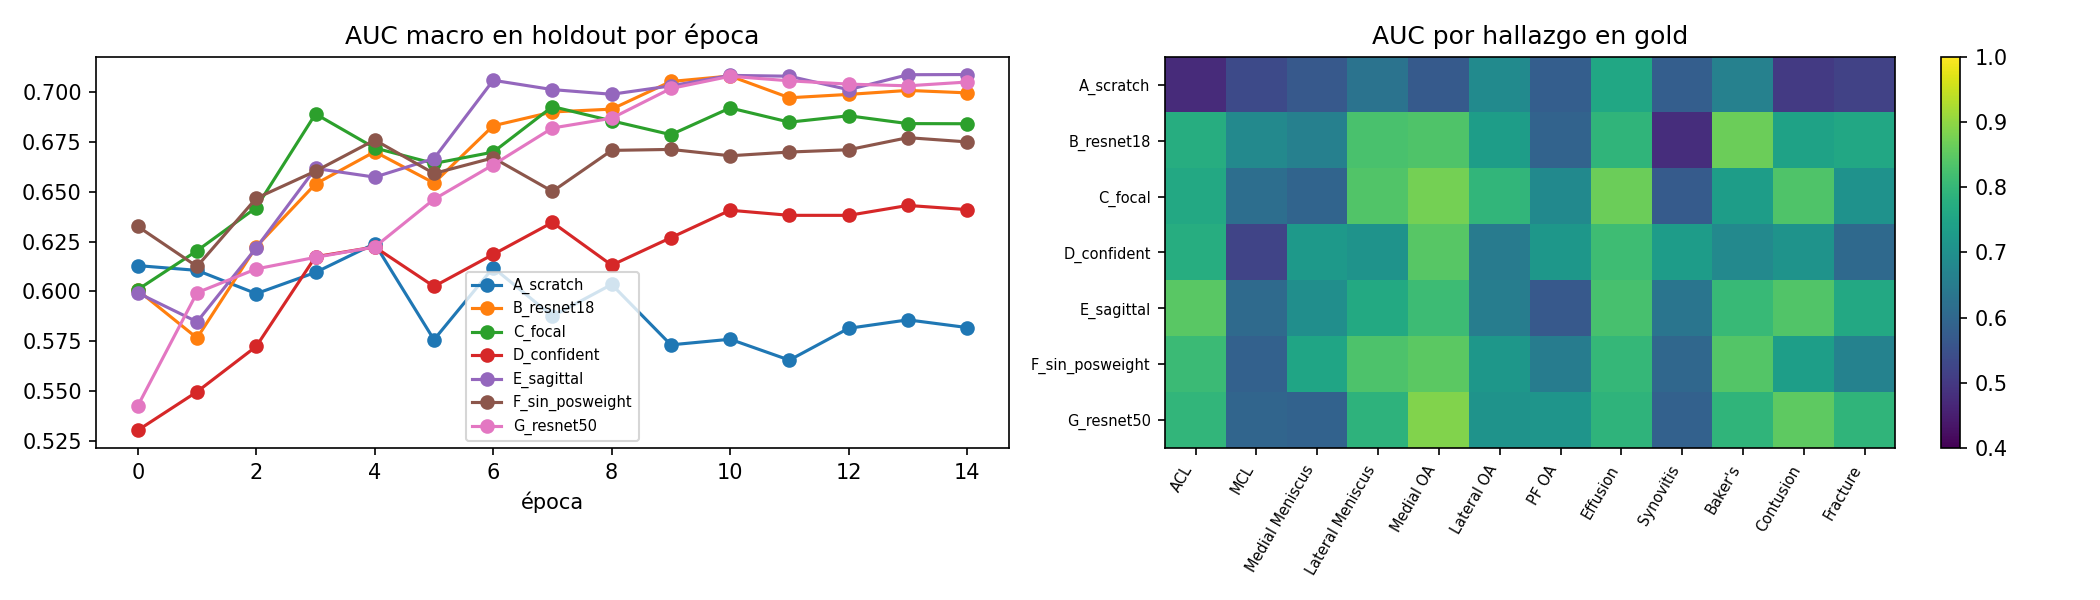
\includegraphics[width=\linewidth]{figs/experimentos.png}
  \caption{Izquierda: AUC macro en el holdout por época. Derecha: AUC por hallazgo en los gold para cada experimento.}
  \label{fig:experimentos}
\end{figure}

\paragraph{Ablaciones (entregable 4).}
Ninguna de las cinco variaciones sobre B produce una diferencia significativa: todos los intervalos de $\Delta$ incluyen el cero.
Con 58 estudios gold, diferencias de AUC menores a $\sim0.04$ no se pueden distinguir del azar, así que las conclusiones siguientes son tendencias.
\begin{itemize}
  \item \textbf{Pérdida} (C, focal~\cite{lin2017focal}, $\gamma=2$): $+0.011$. Es el mejor modelo en derrame ($0.865$) y contusión ($0.835$).
  \item \textbf{Manejo de etiquetas ruidosas} (D): descartar el silencio y las dudas (peso $0$) en lugar de ponderarlos ($0.3$ y $0.5$) baja el AUC macro ($-0.022$), pero cambia mucho según el hallazgo. En sinovitis, D llega a $0.732$ frente a $0.479$ de B. El extractor menciona la sinovitis en solo el $36\%$ de los reportes y el experto la marca en el $47\%$ de los gold, de modo que tratar el silencio como negativo le enseña a B que la sinovitis casi nunca está presente. El mismo efecto, menor, aparece en artrosis patelofemoral ($0.717$ frente a $0.592$) y menisco medial ($0.721$ frente a $0.662$). En cambio, D empeora en MCL, quiste de Baker y fractura, donde descartar el silencio deja muy pocos ejemplos.
  \item \textbf{Plano} (E, solo sagital): rinde igual que los tres planos ($+0.005$) en el $37\%$ del tiempo. El resultado es coherente con la práctica clínica: el ligamento cruzado anterior se evalúa en el plano sagital y E es el mejor modelo en ACL ($0.847$), mientras que pierde en artrosis patelofemoral ($0.568$) y lateral ($0.654$), que se ven mejor en los planos axial y coronal.
  \item \textbf{Profundidad del backbone} (G, ResNet-50): $+0.012$ a 2.6 veces el costo. Es el mejor AUC macro ($0.741$), pero la mejora no es significativa.
\end{itemize}

\begin{table}[t]
  \caption{AUC por hallazgo en los gold. Última columna: el extractor de texto (v4, Sección~\ref{sec:extractor}), que generó las etiquetas de entrenamiento.
    $n^{+}$: positivos según el experto.}
  \label{tab:auc-hallazgo}
  \centering
  \small
  \setlength{\tabcolsep}{4pt}
  \begin{tabular}{@{}lrccccccc|c@{}}
    \toprule
    Hallazgo & $n^{+}$ & A & B & C & D & E & F & G & Texto \\
    \midrule
    ACL              & 24 & .474 & .775 & .761 & .775 & .847 & .809 & .795 & .885 \\
    MCL              &  9 & .535 & .683 & .617 & .524 & .608 & .587 & .596 & .754 \\
    Medial Meniscus  & 26 & .569 & .662 & .594 & .721 & .696 & .754 & .588 & .752 \\
    Lateral Meniscus & 23 & .629 & .827 & .837 & .709 & .764 & .832 & .788 & .806 \\
    Medial OA        & 15 & .571 & .836 & .874 & .843 & .811 & .850 & .885 & .760 \\
    Lateral OA       & 11 & .687 & .733 & .795 & .650 & .654 & .718 & .708 & .733 \\
    PF OA            & 21 & .579 & .592 & .685 & .717 & .568 & .651 & .713 & .690 \\
    Effusion         & 35 & .758 & .793 & .865 & .814 & .825 & .799 & .790 & .666 \\
    Synovitis        & 27 & .579 & .479 & .572 & .732 & .633 & .600 & .587 & .658 \\
    Baker's          & 12 & .663 & .864 & .734 & .683 & .804 & .841 & .792 & .821 \\
    Contusion        & 19 & .502 & .745 & .835 & .707 & .837 & .735 & .852 & .760 \\
    Fracture         & 18 & .519 & .760 & .707 & .606 & .761 & .665 & .793 & .758 \\
    \midrule
    Macro            &    & .589 & .729 & .740 & .707 & .734 & .737 & .741 & .753 \\
    \bottomrule
  \end{tabular}
\end{table}

\paragraph{Resultados por hallazgo (entregable 3).}
La Tabla~\ref{tab:auc-hallazgo} compara cada modelo con el extractor de texto que generó sus etiquetas.
En promedio, el mejor modelo de imagen ($0.741$) queda cerca de su ``maestro'' ($0.753$).
En varios hallazgos lo supera: derrame ($0.865$ en C frente a $0.666$), artrosis medial ($0.885$ en G frente a $0.760$), contusión ($0.852$ en G frente a $0.760$) y menisco lateral ($0.837$ en C frente a $0.806$).
Un modelo entrenado con etiquetas ruidosas puede superar a la fuente de esas etiquetas cuando el ruido no es sistemático, porque la red promedia los errores individuales~\cite{ratner2017snorkel}.
Para ACL, MCL y sinovitis ocurre lo contrario: el reporte describe el hallazgo de forma más directa de lo que la imagen permite aprender con 540 estudios.
El AUC por hallazgo se apoya en 9 a 35 positivos, por lo que sus intervalos son amplios (no mostrados).

\paragraph{Umbral y métricas de decisión.}
El modelo final se elige sin mirar los gold: es el de mejor AUC en el holdout, \texttt{E\_sagittal} ($0.7087$, empatado en la práctica con B y G).
Para cada hallazgo, el umbral es el que maximiza F1 en el holdout.
Elegirlo en los gold daría métricas optimistas, porque se estaría ajustando sobre el mismo conjunto en que se evalúa.
La Tabla~\ref{tab:prf} muestra el resultado.
El recall medio ($0.73$) es mayor que la precisión ($0.47$) porque la prevalencia de los gold difiere de la del entrenamiento (Tabla~\ref{tab:prevalencia}).
Un umbral elegido con la prevalencia débil no se traslada bien a los gold: en sinovitis y fractura, que son mucho más frecuentes en los gold, el recall cae a $0.22$ y $0.33$.

\begin{table}[t]
  \caption{Modelo final (\texttt{E\_sagittal}, elegido por holdout) en los gold, con umbrales que maximizan F1 en el holdout.}
  \label{tab:prf}
  \centering
  \small
  \begin{tabular}{@{}lcccccc@{}}
    \toprule
    Hallazgo & Prevalencia gold & AUC & Umbral & Precisión & Recall & F1 \\
    \midrule
    ACL              & .414 & .847 & .64 & .750 & .750 & .750 \\
    MCL              & .155 & .608 & .53 & .167 & .444 & .242 \\
    Medial Meniscus  & .448 & .696 & .20 & .491 & 1.00 & .658 \\
    Lateral Meniscus & .397 & .764 & .08 & .543 & .826 & .655 \\
    Medial OA        & .259 & .811 & .26 & .361 & .867 & .510 \\
    Lateral OA       & .190 & .654 & .11 & .211 & .727 & .327 \\
    PF OA            & .362 & .568 & .20 & .358 & .905 & .514 \\
    Effusion         & .603 & .825 & .43 & .660 & .943 & .776 \\
    Synovitis        & .466 & .633 & .61 & .667 & .222 & .333 \\
    Baker's          & .207 & .804 & .27 & .300 & 1.00 & .462 \\
    Contusion        & .328 & .837 & .78 & .600 & .789 & .682 \\
    Fracture         & .310 & .761 & .84 & .545 & .333 & .414 \\
    \midrule
    Media            &      & .734 &     & .471 & .734 & .527 \\
    \bottomrule
  \end{tabular}
\end{table}

\begin{table}[t]
  \caption{Prevalencia por hallazgo: etiquetas débiles (train y holdout, puntaje $\geq 0.5$) frente a los gold.}
  \label{tab:prevalencia}
  \centering
  \small
  \begin{tabular}{@{}lcccr@{}}
    \toprule
    Hallazgo & Train (débil) & Holdout (débil) & Gold & $n^{+}$ gold \\
    \midrule
    Fracture         & .128 & .083 & .310 & 18 \\
    Contusion        & .167 & .183 & .328 & 19 \\
    MCL              & .193 & .183 & .155 &  9 \\
    Lateral Meniscus & .202 & .283 & .397 & 23 \\
    Synovitis        & .226 & .217 & .466 & 27 \\
    ACL              & .231 & .317 & .414 & 24 \\
    Baker's          & .283 & .350 & .207 & 12 \\
    Lateral OA       & .359 & .500 & .190 & 11 \\
    Medial Meniscus  & .415 & .500 & .448 & 26 \\
    Medial OA        & .431 & .450 & .259 & 15 \\
    PF OA            & .481 & .650 & .362 & 21 \\
    Effusion         & .613 & .617 & .603 & 35 \\
    \bottomrule
  \end{tabular}
\end{table}

\paragraph{Desbalance de clases (entregable 6).}
En las etiquetas débiles de entrenamiento, la prevalencia va del $13\%$ (fractura) al $61\%$ (derrame) (Tabla~\ref{tab:prevalencia}).
Como mitigación principal, la BCE usa \texttt{pos\_weight} $=(1-p)/p$ por hallazgo, acotado a $[1, 10]$; como alternativa se evaluó la pérdida focal.
Quitar \texttt{pos\_weight} (F) no empeora el AUC ($+0.008$).
Esto es esperable: el AUC solo mide el orden de los casos, y \texttt{pos\_weight} sobre todo desplaza la calibración, lo que aquí se compensa al elegir el umbral en el holdout.
F tiene más recall y menos precisión que B.
La focal (C) da una mejora pequeña y no significativa.
El desbalance que más afecta al resultado no es el interno, sino el desplazamiento entre las etiquetas débiles y los gold.
Fractura, contusión y sinovitis tienen en los gold el doble de prevalencia que en el entrenamiento, y las artrosis lateral y medial casi la mitad.
Los gold parecen haber sido elegidos con más patología, y además el extractor sub-registra los hallazgos que el reporte omite.

\begin{figure}[t]
  \centering
  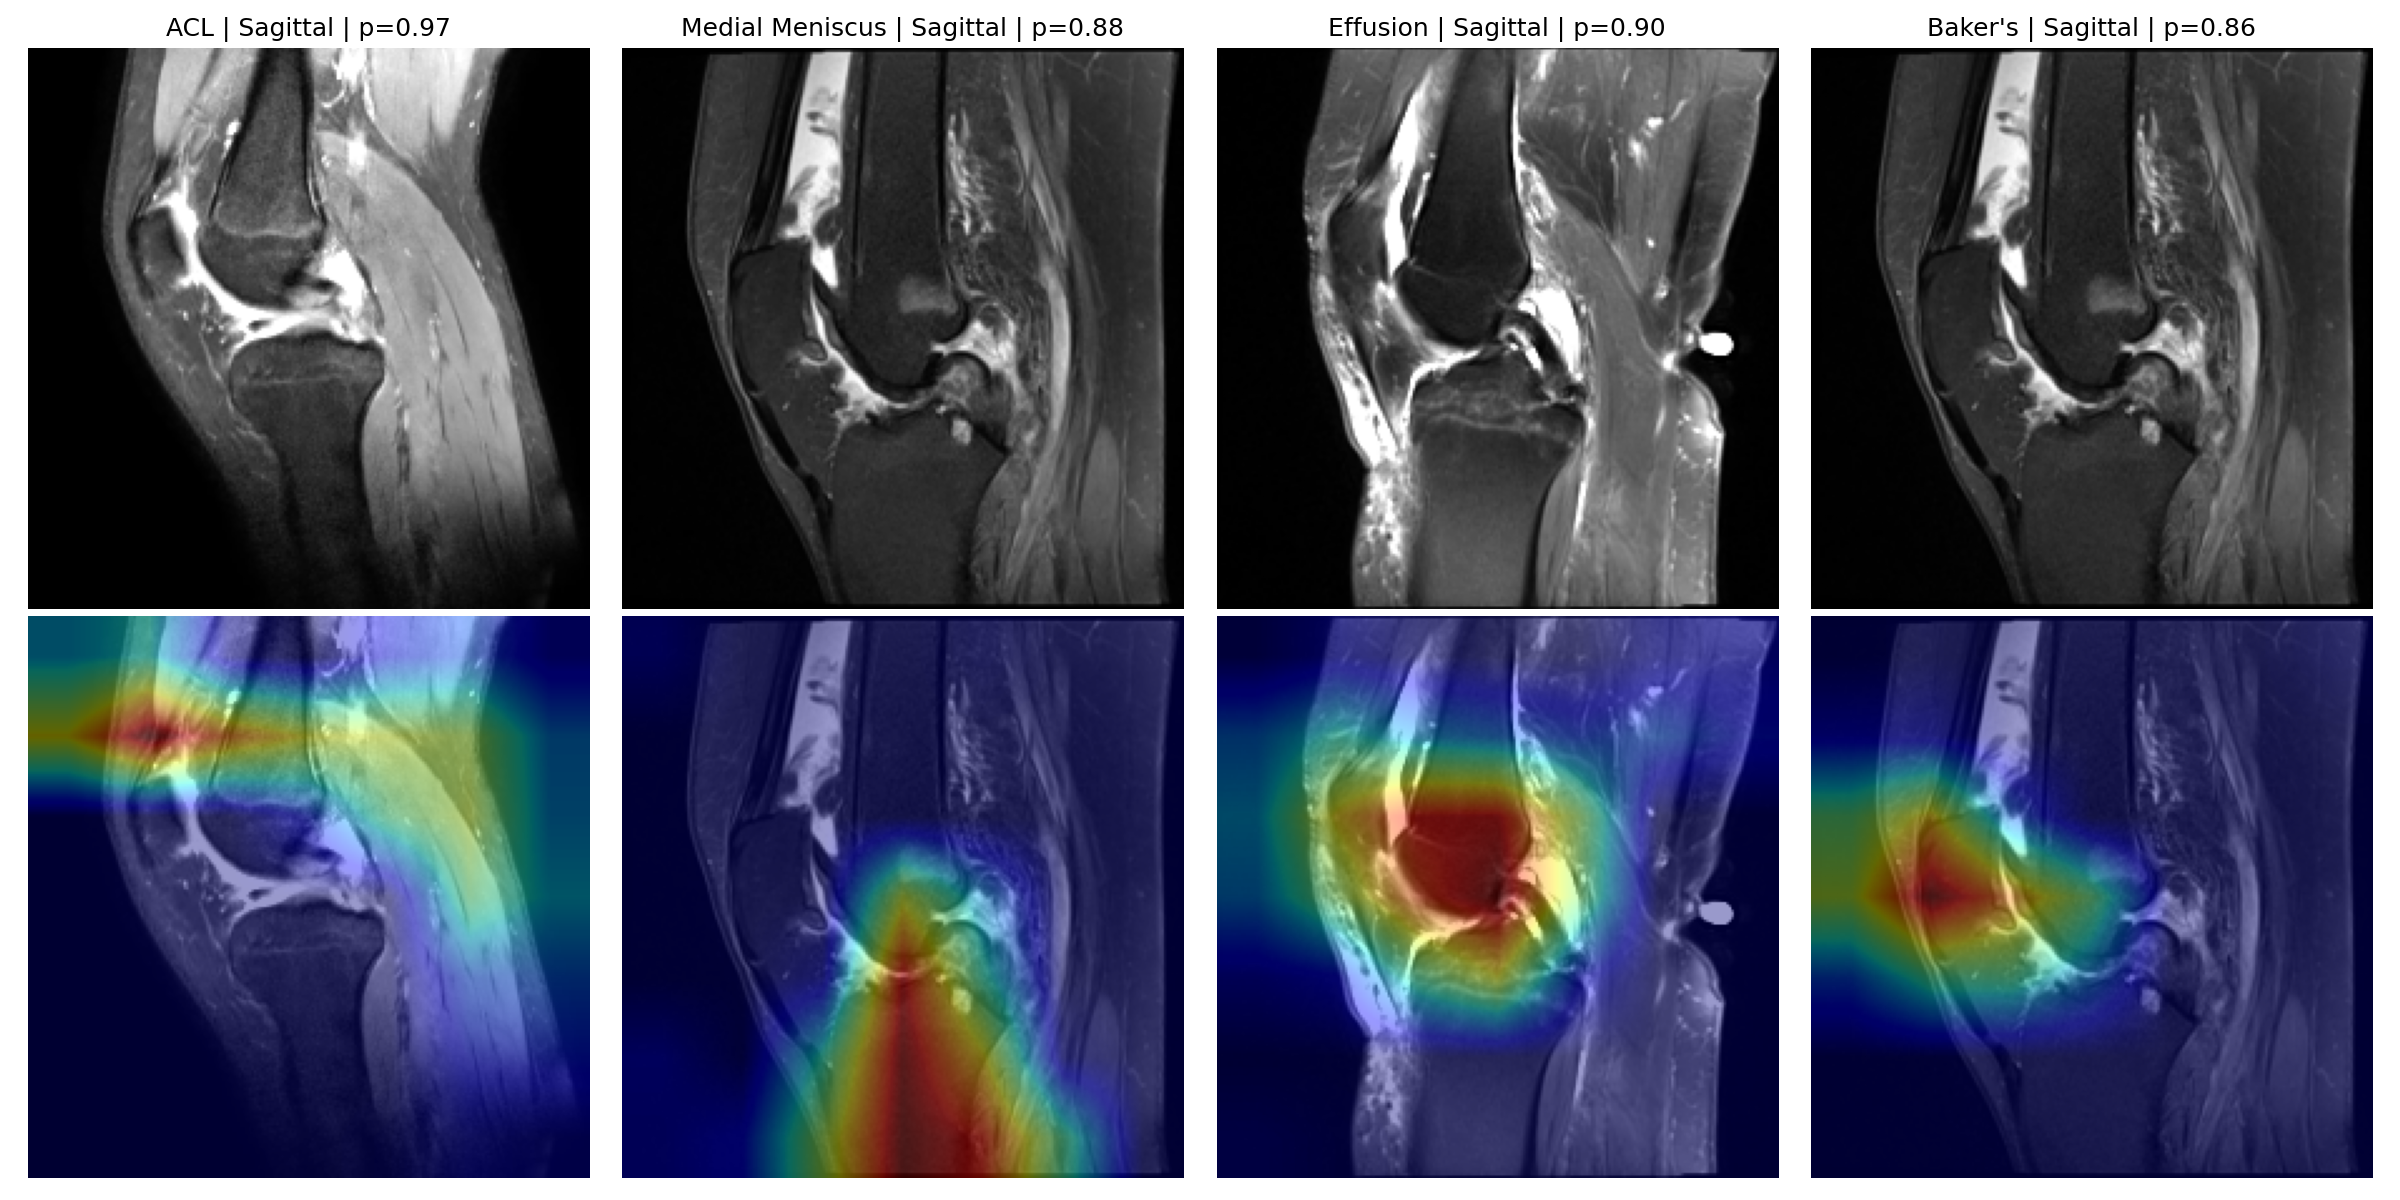
\includegraphics[width=\linewidth]{figs/gradcam.png}
  \caption{Grad-CAM del modelo final (\texttt{E\_sagittal}) sobre la última capa convolucional, en la ventana con mayor atención para cada hallazgo y un estudio gold positivo.
    En las imágenes, anterior está a la izquierda.}
  \label{fig:gradcam}
\end{figure}

\paragraph{Interpretabilidad (entregable 5).}
La Figura~\ref{fig:gradcam} aplica Grad-CAM~\cite{selvaraju2017gradcam} a cuatro hallazgos.
Solo el mapa del derrame es anatómicamente plausible: cubre la cavidad articular y el receso anterior al fémur.
El del menisco medial parte de la línea articular, donde está el menisco, pero se extiende hacia la diáfisis tibial.
Los de ACL y quiste de Baker no señalan la estructura correcta.
El de ACL se concentra en la región suprarrotuliana anterior y no en la escotadura intercondílea.
El de Baker se concentra en la grasa de Hoffa, en la cara anterior, mientras que el quiste poplíteo es posterior.
En la corrida de prueba de una época, el mapa de Baker también apuntaba a la región anterior.
Una explicación plausible es un atajo por co-ocurrencia.
La rotura aguda de ACL suele acompañarse de derrame (hemartrosis), y el quiste de Baker comunica con el líquido articular.
Como las etiquetas débiles salen del mismo reporte, el modelo puede aprender a predecir esos hallazgos a partir del líquido articular, que es más fácil de ver.
El AUC de ACL ($0.847$) sería entonces en parte un efecto de correlación y no de reconocer el ligamento.
Además, la resolución de Grad-CAM en la última capa de ResNet es de $7\times7$, por lo que la localización es gruesa.
   (requiere \usepackage{booktabs} y \usepackage{graphicx})
% Fuente de los números: output-train/ (versión de knee-train del 27 oct 2026, GPU T4, 15 épocas, 49 min en total).

\section{Experimentos}
\label{sec:experimentos}

\paragraph{Protocolo.}
Del total de estudios sin etiqueta experta se tomó un subconjunto estratificado de 600: se incluyen primero los positivos débiles de los hallazgos raros.
De ellos, 540 se usan para entrenar y 60 forman un \emph{holdout}; la partición se hace por reporte, para que dos estudios con el mismo texto no queden en lados distintos.
El holdout tiene solo etiquetas débiles y se usa para elegir la época y los umbrales.
Los 58 estudios gold se excluyen del entrenamiento y solo se usan para la evaluación final.
Cada estudio se representa con una serie por plano (sagital, coronal y axial), 16 cortes de $224\times224$ y ventanas 2.5D de tres cortes vecinos.
En entrenamiento se muestrean 8 ventanas por plano; en evaluación se usan todas.
Los aumentos son rotación $\pm10^\circ$, escala $\pm10\%$ y gamma, sin espejado horizontal (medial y lateral son parte del diagnóstico).
La optimización usa AdamW (tasa $10^{-4}$ en el \emph{backbone} y $10^{-3}$ en la cabeza, \emph{weight decay} $10^{-2}$), calentamiento del $5\%$, decaimiento coseno, recorte de gradiente en $1$ y precisión mixta.
Se entrena 15 épocas con lotes de 8 (4 para ResNet-50) y se conserva la época con mejor AUC macro en el holdout.
Los 7 experimentos tardaron 49 min en una GPU T4.
Los intervalos de confianza (IC 95\%) se obtienen con 1000 remuestreos \emph{bootstrap} de los 58 estudios gold; para las diferencias se usa un bootstrap pareado contra la referencia \texttt{B\_resnet18}.

\begin{table}[t]
  \caption{Resultados en los 58 estudios gold. $\Delta$: diferencia de AUC macro contra la referencia B, con IC 95\% pareado.
    F1 macro con el umbral elegido en el holdout. Época: la de mejor AUC en holdout (de 0 a 14).}
  \label{tab:experimentos}
  \centering
  \small
  \setlength{\tabcolsep}{4pt}
  \begin{tabular}{@{}llccccccc@{}}
    \toprule
    & Variación & AUC gold & IC 95\% & $\Delta$ vs B & IC 95\% $\Delta$ & F1 & Época & Min \\
    \midrule
    A & CNN desde cero         & .589 & [.525, .647] & $-.140$ & [$-.198$, $-.078$] & .447 &  4 &  5.8 \\
    B & ResNet-18 ImageNet (ref.) & .729 & [.673, .782] & ---  & ---                  & .554 & 10 &  5.1 \\
    C & pérdida focal          & .740 & [.686, .789] & $+.011$ & [$-.017$, $+.040$] & .550 &  7 &  5.1 \\
    D & solo etiquetas seguras & .707 & [.648, .761] & $-.022$ & [$-.064$, $+.020$] & .530 & 13 &  5.1 \\
    E & solo plano sagital     & .734 & [.681, .784] & $+.005$ & [$-.046$, $+.052$] & .527 & 14 &  1.9 \\
    F & sin \texttt{pos\_weight} & .737 & [.684, .787] & $+.008$ & [$-.023$, $+.040$] & .553 & 13 &  5.1 \\
    G & ResNet-50 ImageNet     & .741 & [.690, .793] & $+.012$ & [$-.021$, $+.048$] & .551 & 10 & 13.4 \\
    \bottomrule
  \end{tabular}
\end{table}

\paragraph{CNN desde cero frente a transfer learning (entregable 2).}
Ambas arquitecturas comparten la cabeza (proyección, codificación de plano y posición, dos bloques de autoatención y 12 consultas de atención, una por hallazgo, con 12 sigmoides independientes) y solo cambian el extractor de rasgos.
La CNN desde cero (A, 3.1 M parámetros, 5 bloques estilo VGG~\cite{simonyan2015vgg}) obtiene un AUC de $0.589$.
ResNet-18 preentrenada en ImageNet~\cite{he2016resnet} (B, 13.2 M parámetros) llega a $0.729$.
La diferencia, $-0.140$ [$-0.198$, $-0.078$], es la única de la Tabla~\ref{tab:experimentos} cuyo intervalo excluye el cero.
La Figura~\ref{fig:experimentos} muestra por qué: la CNN desde cero alcanza su mejor holdout en la época 4 y luego se estanca alrededor de $0.58$, aunque su pérdida de entrenamiento sigue bajando lentamente.
Con 540 estudios y etiquetas ruidosas no aprende rasgos que generalicen.
Los modelos preentrenados mejoran hasta las épocas 7--10 y luego se estabilizan, lo que indica que 15 épocas fueron suficientes.

\begin{figure}[t]
  \centering
  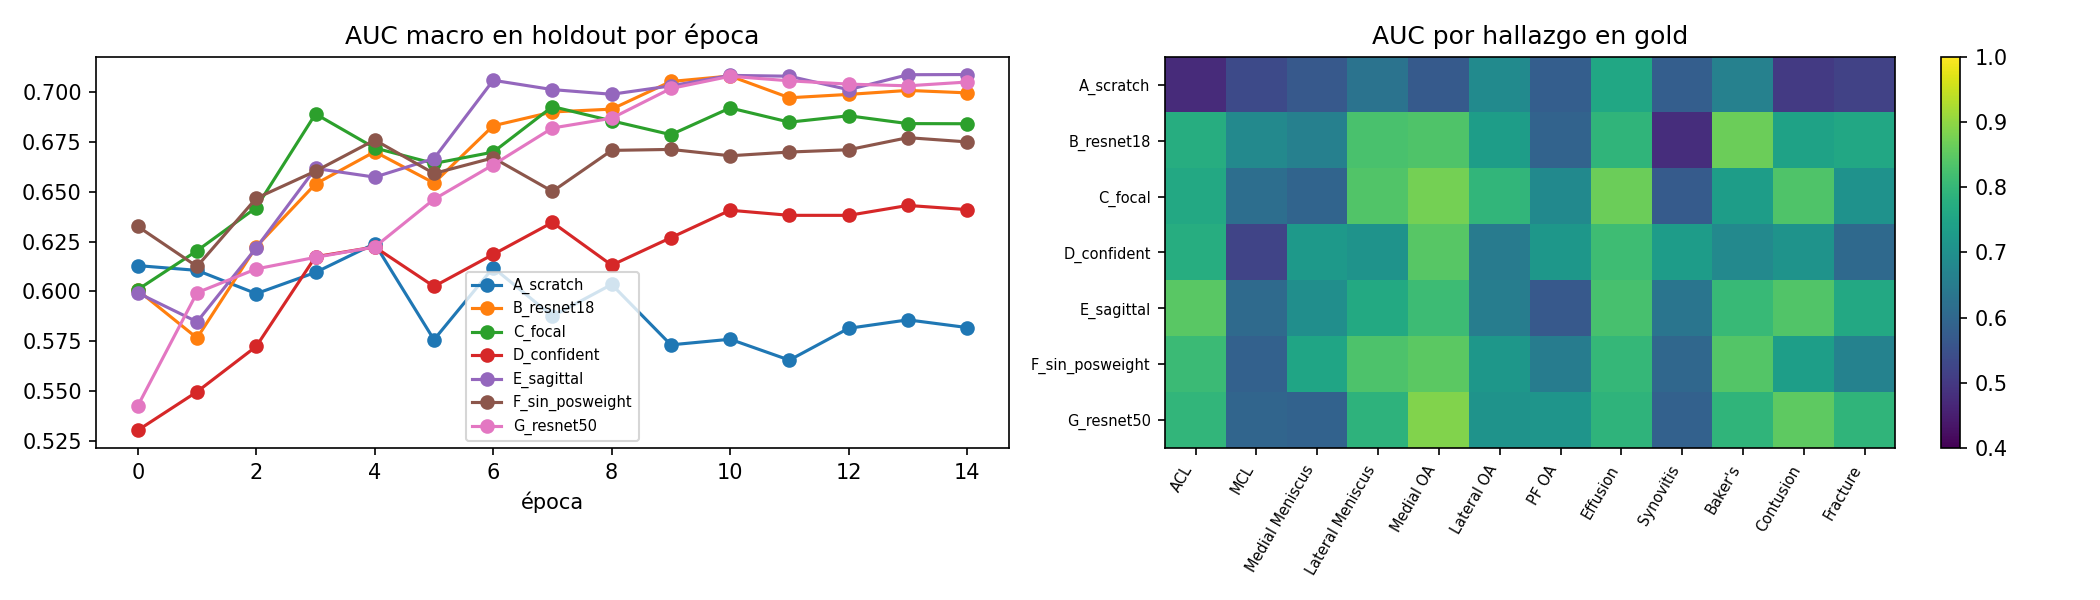
\includegraphics[width=\linewidth]{figs/experimentos.png}
  \caption{Izquierda: AUC macro en el holdout por época. Derecha: AUC por hallazgo en los gold para cada experimento.}
  \label{fig:experimentos}
\end{figure}

\paragraph{Ablaciones (entregable 4).}
Ninguna de las cinco variaciones sobre B produce una diferencia significativa: todos los intervalos de $\Delta$ incluyen el cero.
Con 58 estudios gold, diferencias de AUC menores a $\sim0.04$ no se pueden distinguir del azar, así que las conclusiones siguientes son tendencias.
\begin{itemize}
  \item \textbf{Pérdida} (C, focal~\cite{lin2017focal}, $\gamma=2$): $+0.011$. Es el mejor modelo en derrame ($0.865$) y contusión ($0.835$).
  \item \textbf{Manejo de etiquetas ruidosas} (D): descartar el silencio y las dudas (peso $0$) en lugar de ponderarlos ($0.3$ y $0.5$) baja el AUC macro ($-0.022$), pero cambia mucho según el hallazgo. En sinovitis, D llega a $0.732$ frente a $0.479$ de B. El extractor menciona la sinovitis en solo el $36\%$ de los reportes y el experto la marca en el $47\%$ de los gold, de modo que tratar el silencio como negativo le enseña a B que la sinovitis casi nunca está presente. El mismo efecto, menor, aparece en artrosis patelofemoral ($0.717$ frente a $0.592$) y menisco medial ($0.721$ frente a $0.662$). En cambio, D empeora en MCL, quiste de Baker y fractura, donde descartar el silencio deja muy pocos ejemplos.
  \item \textbf{Plano} (E, solo sagital): rinde igual que los tres planos ($+0.005$) en el $37\%$ del tiempo. El resultado es coherente con la práctica clínica: el ligamento cruzado anterior se evalúa en el plano sagital y E es el mejor modelo en ACL ($0.847$), mientras que pierde en artrosis patelofemoral ($0.568$) y lateral ($0.654$), que se ven mejor en los planos axial y coronal.
  \item \textbf{Profundidad del backbone} (G, ResNet-50): $+0.012$ a 2.6 veces el costo. Es el mejor AUC macro ($0.741$), pero la mejora no es significativa.
\end{itemize}

\begin{table}[t]
  \caption{AUC por hallazgo en los gold. Última columna: el extractor de texto (v4, Sección~\ref{sec:extractor}), que generó las etiquetas de entrenamiento.
    $n^{+}$: positivos según el experto.}
  \label{tab:auc-hallazgo}
  \centering
  \small
  \setlength{\tabcolsep}{4pt}
  \begin{tabular}{@{}lrccccccc|c@{}}
    \toprule
    Hallazgo & $n^{+}$ & A & B & C & D & E & F & G & Texto \\
    \midrule
    ACL              & 24 & .474 & .775 & .761 & .775 & .847 & .809 & .795 & .885 \\
    MCL              &  9 & .535 & .683 & .617 & .524 & .608 & .587 & .596 & .754 \\
    Medial Meniscus  & 26 & .569 & .662 & .594 & .721 & .696 & .754 & .588 & .752 \\
    Lateral Meniscus & 23 & .629 & .827 & .837 & .709 & .764 & .832 & .788 & .806 \\
    Medial OA        & 15 & .571 & .836 & .874 & .843 & .811 & .850 & .885 & .760 \\
    Lateral OA       & 11 & .687 & .733 & .795 & .650 & .654 & .718 & .708 & .733 \\
    PF OA            & 21 & .579 & .592 & .685 & .717 & .568 & .651 & .713 & .690 \\
    Effusion         & 35 & .758 & .793 & .865 & .814 & .825 & .799 & .790 & .666 \\
    Synovitis        & 27 & .579 & .479 & .572 & .732 & .633 & .600 & .587 & .658 \\
    Baker's          & 12 & .663 & .864 & .734 & .683 & .804 & .841 & .792 & .821 \\
    Contusion        & 19 & .502 & .745 & .835 & .707 & .837 & .735 & .852 & .760 \\
    Fracture         & 18 & .519 & .760 & .707 & .606 & .761 & .665 & .793 & .758 \\
    \midrule
    Macro            &    & .589 & .729 & .740 & .707 & .734 & .737 & .741 & .753 \\
    \bottomrule
  \end{tabular}
\end{table}

\paragraph{Resultados por hallazgo (entregable 3).}
La Tabla~\ref{tab:auc-hallazgo} compara cada modelo con el extractor de texto que generó sus etiquetas.
En promedio, el mejor modelo de imagen ($0.741$) queda cerca de su ``maestro'' ($0.753$).
En varios hallazgos lo supera: derrame ($0.865$ en C frente a $0.666$), artrosis medial ($0.885$ en G frente a $0.760$), contusión ($0.852$ en G frente a $0.760$) y menisco lateral ($0.837$ en C frente a $0.806$).
Un modelo entrenado con etiquetas ruidosas puede superar a la fuente de esas etiquetas cuando el ruido no es sistemático, porque la red promedia los errores individuales~\cite{ratner2017snorkel}.
Para ACL, MCL y sinovitis ocurre lo contrario: el reporte describe el hallazgo de forma más directa de lo que la imagen permite aprender con 540 estudios.
El AUC por hallazgo se apoya en 9 a 35 positivos, por lo que sus intervalos son amplios (no mostrados).

\paragraph{Umbral y métricas de decisión.}
El modelo final se elige sin mirar los gold: es el de mejor AUC en el holdout, \texttt{E\_sagittal} ($0.7087$, empatado en la práctica con B y G).
Para cada hallazgo, el umbral es el que maximiza F1 en el holdout.
Elegirlo en los gold daría métricas optimistas, porque se estaría ajustando sobre el mismo conjunto en que se evalúa.
La Tabla~\ref{tab:prf} muestra el resultado.
El recall medio ($0.73$) es mayor que la precisión ($0.47$) porque la prevalencia de los gold difiere de la del entrenamiento (Tabla~\ref{tab:prevalencia}).
Un umbral elegido con la prevalencia débil no se traslada bien a los gold: en sinovitis y fractura, que son mucho más frecuentes en los gold, el recall cae a $0.22$ y $0.33$.

\begin{table}[t]
  \caption{Modelo final (\texttt{E\_sagittal}, elegido por holdout) en los gold, con umbrales que maximizan F1 en el holdout.}
  \label{tab:prf}
  \centering
  \small
  \begin{tabular}{@{}lcccccc@{}}
    \toprule
    Hallazgo & Prevalencia gold & AUC & Umbral & Precisión & Recall & F1 \\
    \midrule
    ACL              & .414 & .847 & .64 & .750 & .750 & .750 \\
    MCL              & .155 & .608 & .53 & .167 & .444 & .242 \\
    Medial Meniscus  & .448 & .696 & .20 & .491 & 1.00 & .658 \\
    Lateral Meniscus & .397 & .764 & .08 & .543 & .826 & .655 \\
    Medial OA        & .259 & .811 & .26 & .361 & .867 & .510 \\
    Lateral OA       & .190 & .654 & .11 & .211 & .727 & .327 \\
    PF OA            & .362 & .568 & .20 & .358 & .905 & .514 \\
    Effusion         & .603 & .825 & .43 & .660 & .943 & .776 \\
    Synovitis        & .466 & .633 & .61 & .667 & .222 & .333 \\
    Baker's          & .207 & .804 & .27 & .300 & 1.00 & .462 \\
    Contusion        & .328 & .837 & .78 & .600 & .789 & .682 \\
    Fracture         & .310 & .761 & .84 & .545 & .333 & .414 \\
    \midrule
    Media            &      & .734 &     & .471 & .734 & .527 \\
    \bottomrule
  \end{tabular}
\end{table}

\begin{table}[t]
  \caption{Prevalencia por hallazgo: etiquetas débiles (train y holdout, puntaje $\geq 0.5$) frente a los gold.}
  \label{tab:prevalencia}
  \centering
  \small
  \begin{tabular}{@{}lcccr@{}}
    \toprule
    Hallazgo & Train (débil) & Holdout (débil) & Gold & $n^{+}$ gold \\
    \midrule
    Fracture         & .128 & .083 & .310 & 18 \\
    Contusion        & .167 & .183 & .328 & 19 \\
    MCL              & .193 & .183 & .155 &  9 \\
    Lateral Meniscus & .202 & .283 & .397 & 23 \\
    Synovitis        & .226 & .217 & .466 & 27 \\
    ACL              & .231 & .317 & .414 & 24 \\
    Baker's          & .283 & .350 & .207 & 12 \\
    Lateral OA       & .359 & .500 & .190 & 11 \\
    Medial Meniscus  & .415 & .500 & .448 & 26 \\
    Medial OA        & .431 & .450 & .259 & 15 \\
    PF OA            & .481 & .650 & .362 & 21 \\
    Effusion         & .613 & .617 & .603 & 35 \\
    \bottomrule
  \end{tabular}
\end{table}

\paragraph{Desbalance de clases (entregable 6).}
En las etiquetas débiles de entrenamiento, la prevalencia va del $13\%$ (fractura) al $61\%$ (derrame) (Tabla~\ref{tab:prevalencia}).
Como mitigación principal, la BCE usa \texttt{pos\_weight} $=(1-p)/p$ por hallazgo, acotado a $[1, 10]$; como alternativa se evaluó la pérdida focal.
Quitar \texttt{pos\_weight} (F) no empeora el AUC ($+0.008$).
Esto es esperable: el AUC solo mide el orden de los casos, y \texttt{pos\_weight} sobre todo desplaza la calibración, lo que aquí se compensa al elegir el umbral en el holdout.
F tiene más recall y menos precisión que B.
La focal (C) da una mejora pequeña y no significativa.
El desbalance que más afecta al resultado no es el interno, sino el desplazamiento entre las etiquetas débiles y los gold.
Fractura, contusión y sinovitis tienen en los gold el doble de prevalencia que en el entrenamiento, y las artrosis lateral y medial casi la mitad.
Los gold parecen haber sido elegidos con más patología, y además el extractor sub-registra los hallazgos que el reporte omite.

\begin{figure}[t]
  \centering
  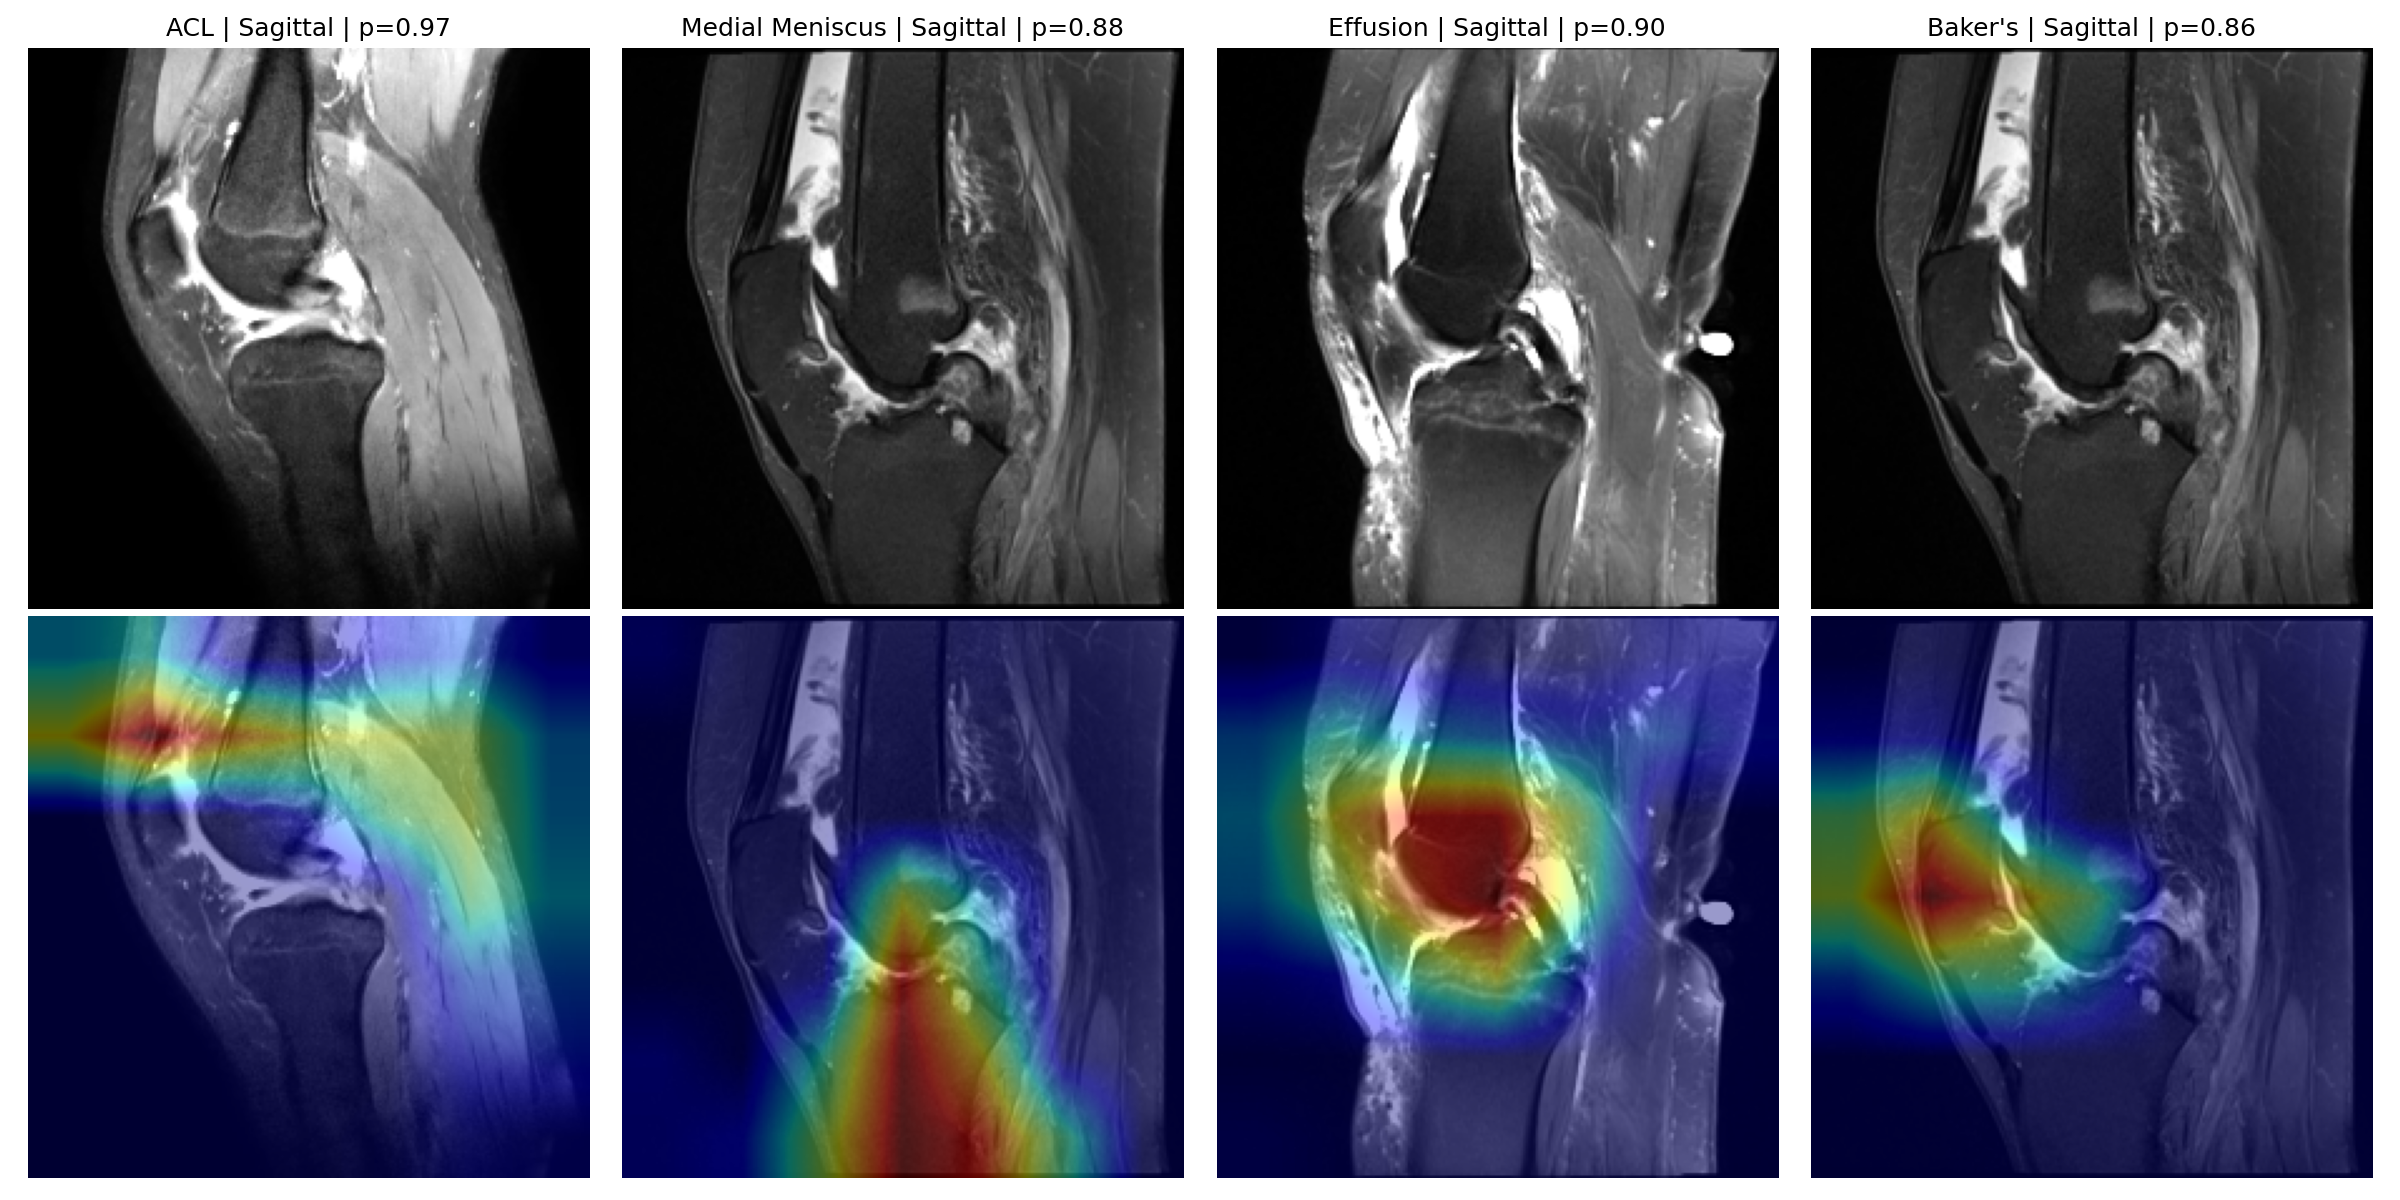
\includegraphics[width=\linewidth]{figs/gradcam.png}
  \caption{Grad-CAM del modelo final (\texttt{E\_sagittal}) sobre la última capa convolucional, en la ventana con mayor atención para cada hallazgo y un estudio gold positivo.
    En las imágenes, anterior está a la izquierda.}
  \label{fig:gradcam}
\end{figure}

\paragraph{Interpretabilidad (entregable 5).}
La Figura~\ref{fig:gradcam} aplica Grad-CAM~\cite{selvaraju2017gradcam} a cuatro hallazgos.
Solo el mapa del derrame es anatómicamente plausible: cubre la cavidad articular y el receso anterior al fémur.
El del menisco medial parte de la línea articular, donde está el menisco, pero se extiende hacia la diáfisis tibial.
Los de ACL y quiste de Baker no señalan la estructura correcta.
El de ACL se concentra en la región suprarrotuliana anterior y no en la escotadura intercondílea.
El de Baker se concentra en la grasa de Hoffa, en la cara anterior, mientras que el quiste poplíteo es posterior.
En la corrida de prueba de una época, el mapa de Baker también apuntaba a la región anterior.
Una explicación plausible es un atajo por co-ocurrencia.
La rotura aguda de ACL suele acompañarse de derrame (hemartrosis), y el quiste de Baker comunica con el líquido articular.
Como las etiquetas débiles salen del mismo reporte, el modelo puede aprender a predecir esos hallazgos a partir del líquido articular, que es más fácil de ver.
El AUC de ACL ($0.847$) sería entonces en parte un efecto de correlación y no de reconocer el ligamento.
Además, la resolución de Grad-CAM en la última capa de ResNet es de $7\times7$, por lo que la localización es gruesa.
   (requiere \usepackage{booktabs} y \usepackage{graphicx})
% Fuente de los números: output-train/ (versión de knee-train del 27 oct 2026, GPU T4, 15 épocas, 49 min en total).

\section{Experimentos}
\label{sec:experimentos}

\paragraph{Protocolo.}
Del total de estudios sin etiqueta experta se tomó un subconjunto estratificado de 600: se incluyen primero los positivos débiles de los hallazgos raros.
De ellos, 540 se usan para entrenar y 60 forman un \emph{holdout}; la partición se hace por reporte, para que dos estudios con el mismo texto no queden en lados distintos.
El holdout tiene solo etiquetas débiles y se usa para elegir la época y los umbrales.
Los 58 estudios gold se excluyen del entrenamiento y solo se usan para la evaluación final.
Cada estudio se representa con una serie por plano (sagital, coronal y axial), 16 cortes de $224\times224$ y ventanas 2.5D de tres cortes vecinos.
En entrenamiento se muestrean 8 ventanas por plano; en evaluación se usan todas.
Los aumentos son rotación $\pm10^\circ$, escala $\pm10\%$ y gamma, sin espejado horizontal (medial y lateral son parte del diagnóstico).
La optimización usa AdamW (tasa $10^{-4}$ en el \emph{backbone} y $10^{-3}$ en la cabeza, \emph{weight decay} $10^{-2}$), calentamiento del $5\%$, decaimiento coseno, recorte de gradiente en $1$ y precisión mixta.
Se entrena 15 épocas con lotes de 8 (4 para ResNet-50) y se conserva la época con mejor AUC macro en el holdout.
Los 7 experimentos tardaron 49 min en una GPU T4.
Los intervalos de confianza (IC 95\%) se obtienen con 1000 remuestreos \emph{bootstrap} de los 58 estudios gold; para las diferencias se usa un bootstrap pareado contra la referencia \texttt{B\_resnet18}.

\begin{table}[t]
  \caption{Resultados en los 58 estudios gold. $\Delta$: diferencia de AUC macro contra la referencia B, con IC 95\% pareado.
    F1 macro con el umbral elegido en el holdout. Época: la de mejor AUC en holdout (de 0 a 14).}
  \label{tab:experimentos}
  \centering
  \small
  \setlength{\tabcolsep}{4pt}
  \begin{tabular}{@{}llccccccc@{}}
    \toprule
    & Variación & AUC gold & IC 95\% & $\Delta$ vs B & IC 95\% $\Delta$ & F1 & Época & Min \\
    \midrule
    A & CNN desde cero         & .589 & [.525, .647] & $-.140$ & [$-.198$, $-.078$] & .447 &  4 &  5.8 \\
    B & ResNet-18 ImageNet (ref.) & .729 & [.673, .782] & ---  & ---                  & .554 & 10 &  5.1 \\
    C & pérdida focal          & .740 & [.686, .789] & $+.011$ & [$-.017$, $+.040$] & .550 &  7 &  5.1 \\
    D & solo etiquetas seguras & .707 & [.648, .761] & $-.022$ & [$-.064$, $+.020$] & .530 & 13 &  5.1 \\
    E & solo plano sagital     & .734 & [.681, .784] & $+.005$ & [$-.046$, $+.052$] & .527 & 14 &  1.9 \\
    F & sin \texttt{pos\_weight} & .737 & [.684, .787] & $+.008$ & [$-.023$, $+.040$] & .553 & 13 &  5.1 \\
    G & ResNet-50 ImageNet     & .741 & [.690, .793] & $+.012$ & [$-.021$, $+.048$] & .551 & 10 & 13.4 \\
    \bottomrule
  \end{tabular}
\end{table}

\paragraph{CNN desde cero frente a transfer learning (entregable 2).}
Ambas arquitecturas comparten la cabeza (proyección, codificación de plano y posición, dos bloques de autoatención y 12 consultas de atención, una por hallazgo, con 12 sigmoides independientes) y solo cambian el extractor de rasgos.
La CNN desde cero (A, 3.1 M parámetros, 5 bloques estilo VGG~\cite{simonyan2015vgg}) obtiene un AUC de $0.589$.
ResNet-18 preentrenada en ImageNet~\cite{he2016resnet} (B, 13.2 M parámetros) llega a $0.729$.
La diferencia, $-0.140$ [$-0.198$, $-0.078$], es la única de la Tabla~\ref{tab:experimentos} cuyo intervalo excluye el cero.
La Figura~\ref{fig:experimentos} muestra por qué: la CNN desde cero alcanza su mejor holdout en la época 4 y luego se estanca alrededor de $0.58$, aunque su pérdida de entrenamiento sigue bajando lentamente.
Con 540 estudios y etiquetas ruidosas no aprende rasgos que generalicen.
Los modelos preentrenados mejoran hasta las épocas 7--10 y luego se estabilizan, lo que indica que 15 épocas fueron suficientes.

\begin{figure}[t]
  \centering
  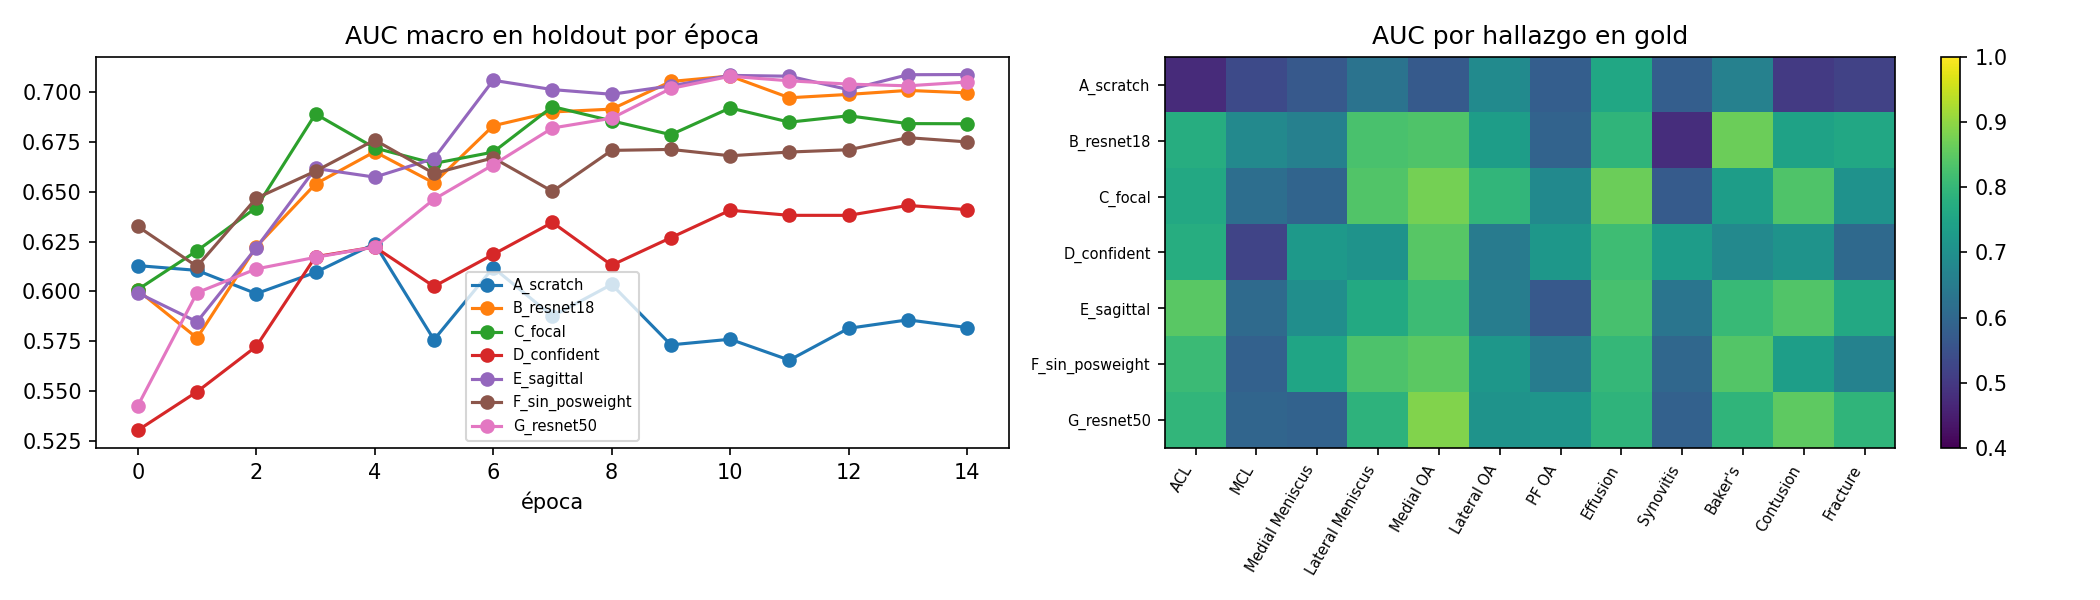
\includegraphics[width=\linewidth]{figs/experimentos.png}
  \caption{Izquierda: AUC macro en el holdout por época. Derecha: AUC por hallazgo en los gold para cada experimento.}
  \label{fig:experimentos}
\end{figure}

\paragraph{Ablaciones (entregable 4).}
Ninguna de las cinco variaciones sobre B produce una diferencia significativa: todos los intervalos de $\Delta$ incluyen el cero.
Con 58 estudios gold, diferencias de AUC menores a $\sim0.04$ no se pueden distinguir del azar, así que las conclusiones siguientes son tendencias.
\begin{itemize}
  \item \textbf{Pérdida} (C, focal~\cite{lin2017focal}, $\gamma=2$): $+0.011$. Es el mejor modelo en derrame ($0.865$) y contusión ($0.835$).
  \item \textbf{Manejo de etiquetas ruidosas} (D): descartar el silencio y las dudas (peso $0$) en lugar de ponderarlos ($0.3$ y $0.5$) baja el AUC macro ($-0.022$), pero cambia mucho según el hallazgo. En sinovitis, D llega a $0.732$ frente a $0.479$ de B. El extractor menciona la sinovitis en solo el $36\%$ de los reportes y el experto la marca en el $47\%$ de los gold, de modo que tratar el silencio como negativo le enseña a B que la sinovitis casi nunca está presente. El mismo efecto, menor, aparece en artrosis patelofemoral ($0.717$ frente a $0.592$) y menisco medial ($0.721$ frente a $0.662$). En cambio, D empeora en MCL, quiste de Baker y fractura, donde descartar el silencio deja muy pocos ejemplos.
  \item \textbf{Plano} (E, solo sagital): rinde igual que los tres planos ($+0.005$) en el $37\%$ del tiempo. El resultado es coherente con la práctica clínica: el ligamento cruzado anterior se evalúa en el plano sagital y E es el mejor modelo en ACL ($0.847$), mientras que pierde en artrosis patelofemoral ($0.568$) y lateral ($0.654$), que se ven mejor en los planos axial y coronal.
  \item \textbf{Profundidad del backbone} (G, ResNet-50): $+0.012$ a 2.6 veces el costo. Es el mejor AUC macro ($0.741$), pero la mejora no es significativa.
\end{itemize}

\begin{table}[t]
  \caption{AUC por hallazgo en los gold. Última columna: el extractor de texto (v4, Sección~\ref{sec:extractor}), que generó las etiquetas de entrenamiento.
    $n^{+}$: positivos según el experto.}
  \label{tab:auc-hallazgo}
  \centering
  \small
  \setlength{\tabcolsep}{4pt}
  \begin{tabular}{@{}lrccccccc|c@{}}
    \toprule
    Hallazgo & $n^{+}$ & A & B & C & D & E & F & G & Texto \\
    \midrule
    ACL              & 24 & .474 & .775 & .761 & .775 & .847 & .809 & .795 & .885 \\
    MCL              &  9 & .535 & .683 & .617 & .524 & .608 & .587 & .596 & .754 \\
    Medial Meniscus  & 26 & .569 & .662 & .594 & .721 & .696 & .754 & .588 & .752 \\
    Lateral Meniscus & 23 & .629 & .827 & .837 & .709 & .764 & .832 & .788 & .806 \\
    Medial OA        & 15 & .571 & .836 & .874 & .843 & .811 & .850 & .885 & .760 \\
    Lateral OA       & 11 & .687 & .733 & .795 & .650 & .654 & .718 & .708 & .733 \\
    PF OA            & 21 & .579 & .592 & .685 & .717 & .568 & .651 & .713 & .690 \\
    Effusion         & 35 & .758 & .793 & .865 & .814 & .825 & .799 & .790 & .666 \\
    Synovitis        & 27 & .579 & .479 & .572 & .732 & .633 & .600 & .587 & .658 \\
    Baker's          & 12 & .663 & .864 & .734 & .683 & .804 & .841 & .792 & .821 \\
    Contusion        & 19 & .502 & .745 & .835 & .707 & .837 & .735 & .852 & .760 \\
    Fracture         & 18 & .519 & .760 & .707 & .606 & .761 & .665 & .793 & .758 \\
    \midrule
    Macro            &    & .589 & .729 & .740 & .707 & .734 & .737 & .741 & .753 \\
    \bottomrule
  \end{tabular}
\end{table}

\paragraph{Resultados por hallazgo (entregable 3).}
La Tabla~\ref{tab:auc-hallazgo} compara cada modelo con el extractor de texto que generó sus etiquetas.
En promedio, el mejor modelo de imagen ($0.741$) queda cerca de su ``maestro'' ($0.753$).
En varios hallazgos lo supera: derrame ($0.865$ en C frente a $0.666$), artrosis medial ($0.885$ en G frente a $0.760$), contusión ($0.852$ en G frente a $0.760$) y menisco lateral ($0.837$ en C frente a $0.806$).
Un modelo entrenado con etiquetas ruidosas puede superar a la fuente de esas etiquetas cuando el ruido no es sistemático, porque la red promedia los errores individuales~\cite{ratner2017snorkel}.
Para ACL, MCL y sinovitis ocurre lo contrario: el reporte describe el hallazgo de forma más directa de lo que la imagen permite aprender con 540 estudios.
El AUC por hallazgo se apoya en 9 a 35 positivos, por lo que sus intervalos son amplios (no mostrados).

\paragraph{Umbral y métricas de decisión.}
El modelo final se elige sin mirar los gold: es el de mejor AUC en el holdout, \texttt{E\_sagittal} ($0.7087$, empatado en la práctica con B y G).
Para cada hallazgo, el umbral es el que maximiza F1 en el holdout.
Elegirlo en los gold daría métricas optimistas, porque se estaría ajustando sobre el mismo conjunto en que se evalúa.
La Tabla~\ref{tab:prf} muestra el resultado.
El recall medio ($0.73$) es mayor que la precisión ($0.47$) porque la prevalencia de los gold difiere de la del entrenamiento (Tabla~\ref{tab:prevalencia}).
Un umbral elegido con la prevalencia débil no se traslada bien a los gold: en sinovitis y fractura, que son mucho más frecuentes en los gold, el recall cae a $0.22$ y $0.33$.

\begin{table}[t]
  \caption{Modelo final (\texttt{E\_sagittal}, elegido por holdout) en los gold, con umbrales que maximizan F1 en el holdout.}
  \label{tab:prf}
  \centering
  \small
  \begin{tabular}{@{}lcccccc@{}}
    \toprule
    Hallazgo & Prevalencia gold & AUC & Umbral & Precisión & Recall & F1 \\
    \midrule
    ACL              & .414 & .847 & .64 & .750 & .750 & .750 \\
    MCL              & .155 & .608 & .53 & .167 & .444 & .242 \\
    Medial Meniscus  & .448 & .696 & .20 & .491 & 1.00 & .658 \\
    Lateral Meniscus & .397 & .764 & .08 & .543 & .826 & .655 \\
    Medial OA        & .259 & .811 & .26 & .361 & .867 & .510 \\
    Lateral OA       & .190 & .654 & .11 & .211 & .727 & .327 \\
    PF OA            & .362 & .568 & .20 & .358 & .905 & .514 \\
    Effusion         & .603 & .825 & .43 & .660 & .943 & .776 \\
    Synovitis        & .466 & .633 & .61 & .667 & .222 & .333 \\
    Baker's          & .207 & .804 & .27 & .300 & 1.00 & .462 \\
    Contusion        & .328 & .837 & .78 & .600 & .789 & .682 \\
    Fracture         & .310 & .761 & .84 & .545 & .333 & .414 \\
    \midrule
    Media            &      & .734 &     & .471 & .734 & .527 \\
    \bottomrule
  \end{tabular}
\end{table}

\begin{table}[t]
  \caption{Prevalencia por hallazgo: etiquetas débiles (train y holdout, puntaje $\geq 0.5$) frente a los gold.}
  \label{tab:prevalencia}
  \centering
  \small
  \begin{tabular}{@{}lcccr@{}}
    \toprule
    Hallazgo & Train (débil) & Holdout (débil) & Gold & $n^{+}$ gold \\
    \midrule
    Fracture         & .128 & .083 & .310 & 18 \\
    Contusion        & .167 & .183 & .328 & 19 \\
    MCL              & .193 & .183 & .155 &  9 \\
    Lateral Meniscus & .202 & .283 & .397 & 23 \\
    Synovitis        & .226 & .217 & .466 & 27 \\
    ACL              & .231 & .317 & .414 & 24 \\
    Baker's          & .283 & .350 & .207 & 12 \\
    Lateral OA       & .359 & .500 & .190 & 11 \\
    Medial Meniscus  & .415 & .500 & .448 & 26 \\
    Medial OA        & .431 & .450 & .259 & 15 \\
    PF OA            & .481 & .650 & .362 & 21 \\
    Effusion         & .613 & .617 & .603 & 35 \\
    \bottomrule
  \end{tabular}
\end{table}

\paragraph{Desbalance de clases (entregable 6).}
En las etiquetas débiles de entrenamiento, la prevalencia va del $13\%$ (fractura) al $61\%$ (derrame) (Tabla~\ref{tab:prevalencia}).
Como mitigación principal, la BCE usa \texttt{pos\_weight} $=(1-p)/p$ por hallazgo, acotado a $[1, 10]$; como alternativa se evaluó la pérdida focal.
Quitar \texttt{pos\_weight} (F) no empeora el AUC ($+0.008$).
Esto es esperable: el AUC solo mide el orden de los casos, y \texttt{pos\_weight} sobre todo desplaza la calibración, lo que aquí se compensa al elegir el umbral en el holdout.
F tiene más recall y menos precisión que B.
La focal (C) da una mejora pequeña y no significativa.
El desbalance que más afecta al resultado no es el interno, sino el desplazamiento entre las etiquetas débiles y los gold.
Fractura, contusión y sinovitis tienen en los gold el doble de prevalencia que en el entrenamiento, y las artrosis lateral y medial casi la mitad.
Los gold parecen haber sido elegidos con más patología, y además el extractor sub-registra los hallazgos que el reporte omite.

\begin{figure}[t]
  \centering
  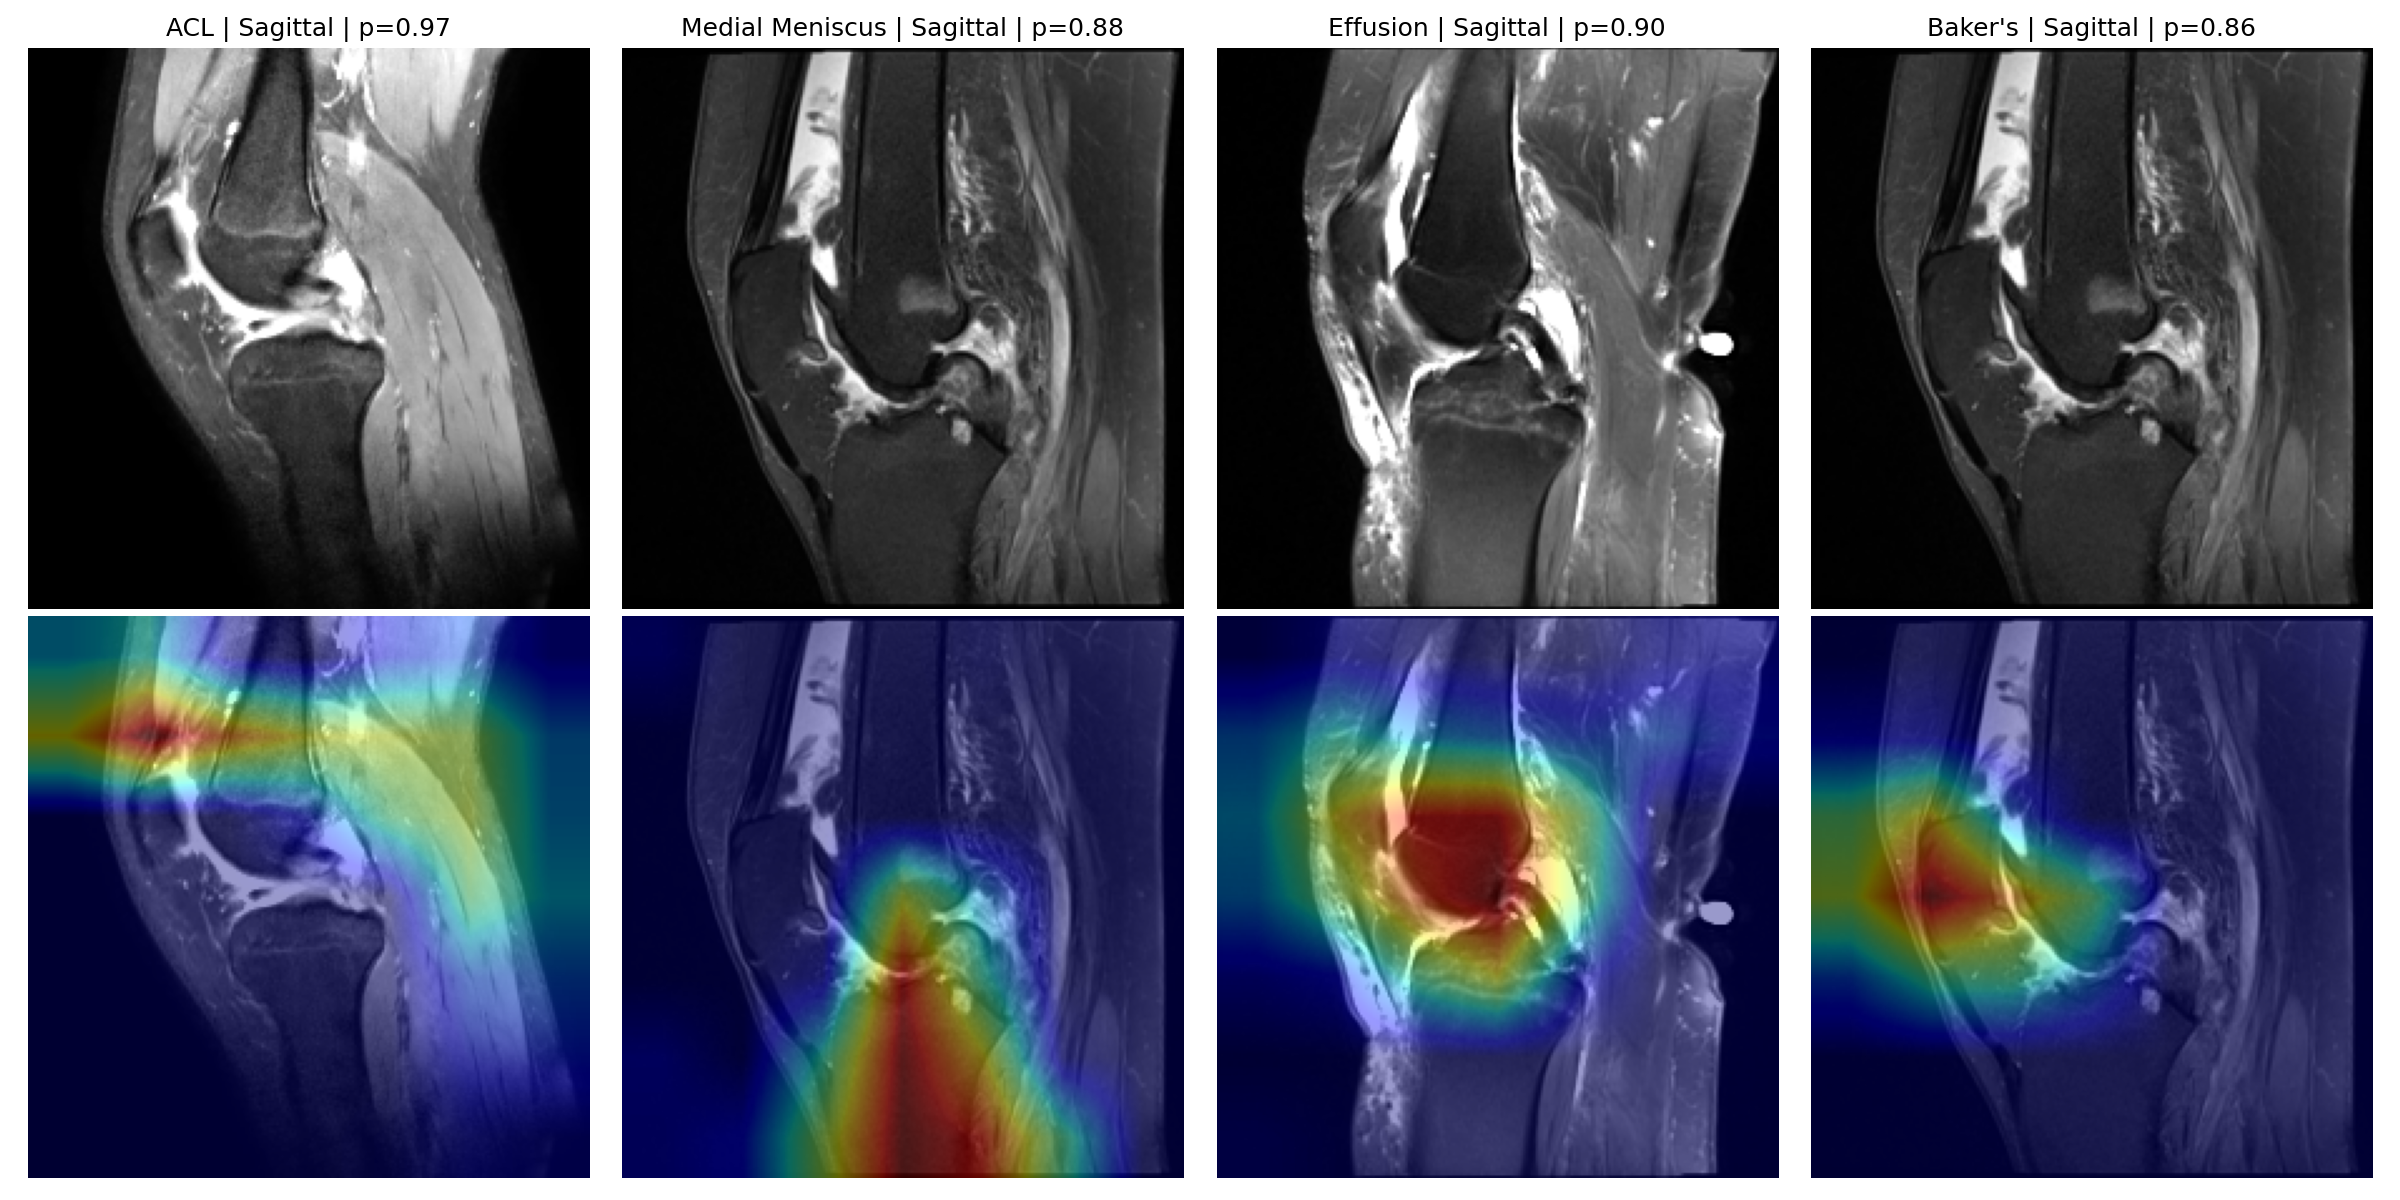
\includegraphics[width=\linewidth]{figs/gradcam.png}
  \caption{Grad-CAM del modelo final (\texttt{E\_sagittal}) sobre la última capa convolucional, en la ventana con mayor atención para cada hallazgo y un estudio gold positivo.
    En las imágenes, anterior está a la izquierda.}
  \label{fig:gradcam}
\end{figure}

\paragraph{Interpretabilidad (entregable 5).}
La Figura~\ref{fig:gradcam} aplica Grad-CAM~\cite{selvaraju2017gradcam} a cuatro hallazgos.
Solo el mapa del derrame es anatómicamente plausible: cubre la cavidad articular y el receso anterior al fémur.
El del menisco medial parte de la línea articular, donde está el menisco, pero se extiende hacia la diáfisis tibial.
Los de ACL y quiste de Baker no señalan la estructura correcta.
El de ACL se concentra en la región suprarrotuliana anterior y no en la escotadura intercondílea.
El de Baker se concentra en la grasa de Hoffa, en la cara anterior, mientras que el quiste poplíteo es posterior.
En la corrida de prueba de una época, el mapa de Baker también apuntaba a la región anterior.
Una explicación plausible es un atajo por co-ocurrencia.
La rotura aguda de ACL suele acompañarse de derrame (hemartrosis), y el quiste de Baker comunica con el líquido articular.
Como las etiquetas débiles salen del mismo reporte, el modelo puede aprender a predecir esos hallazgos a partir del líquido articular, que es más fácil de ver.
El AUC de ACL ($0.847$) sería entonces en parte un efecto de correlación y no de reconocer el ligamento.
Además, la resolución de Grad-CAM en la última capa de ResNet es de $7\times7$, por lo que la localización es gruesa.
